\documentclass[11pt]{article}

\usepackage[T1]{fontenc}
\usepackage{lmodern}
\usepackage[margin=1in]{geometry}
\usepackage{amsmath,amssymb}
\usepackage{mathtools}
\usepackage{array,booktabs,tabularx}
\usepackage{adjustbox}
\usepackage{graphicx}
\usepackage{float}
\usepackage{xcolor}
\usepackage{microtype}
\usepackage[numbers,sort&compress]{natbib}
\usepackage{hyperref}
\usepackage{listings}
\usepackage{tikz}
\usepackage{placeins}
\usepackage{graphcore_bwd_report}
\usetikzlibrary{arrows.meta,positioning,fit}

\setlength{\parindent}{0pt}
\setlength{\parskip}{0.55em}
\setlength{\emergencystretch}{2em}
\renewcommand{\arraystretch}{1.14}
\newcolumntype{Y}{>{\raggedright\arraybackslash}X}

\floatstyle{ruled}
\newfloat{algorithm}{tbp}{loa}
\floatname{algorithm}{Algorithm}
\restylefloat{algorithm}

\title{Hardware-Aware FP4 FlashAttention-4 Backward}
\reportsubtitle{Adaptive low-precision gradients and unified QKV projection integration}
\author{Robert Hu}
\date{August 2026}
\hypersetup{
  colorlinks=true,
  linkcolor=GraphcoreInk,
  citecolor=GraphcoreCoralDark,
  urlcolor=GraphcoreCoralDark,
  pdftitle={Hardware-Aware FP4 FlashAttention-4 Backward},
  pdfauthor={Robert Hu},
  pdfsubject={Adaptive FP4 FlashAttention-4 backward and unified QKV projection integration on NVIDIA Blackwell},
  pdfkeywords={FlashAttention-4, backward, FP4, FP8, NVFP4, MXFP4, Blackwell, tensor memory, projection}
}

\definecolor{scoreblue}{HTML}{2A6FBB}
\definecolor{outputgreen}{HTML}{28865D}
\definecolor{probred}{HTML}{C83E4D}
\definecolor{scaleyellow}{HTML}{D99B22}
\definecolor{inkgray}{HTML}{3C4650}
\definecolor{lightgray}{HTML}{EDF0F2}
\definecolor{gradientpurple}{HTML}{7452A8}

\newcommand{\E}{\mathbb{E}}
\newcommand{\R}{\mathbb{R}}
\newcommand{\softmax}{\operatorname{softmax}}
\newcommand{\Qfour}{Q_{\mathrm{E2M1}}}
\newcommand{\Qeight}{Q_{\mathrm{E4M3}}}
\newcommand{\code}[1]{\texttt{#1}}
\newcommand{\us}{\ensuremath{\,\mu\mathrm{s}}}
\newcommand{\tmem}{\textsc{tmem}}
\newcommand{\smem}{\textsc{smem}}
\newcommand{\hbm}{\textsc{hbm}}
\newcommand{\tcgen}{\texttt{tcgen05}}
\newcommand{\mma}{\operatorname{MMA}}
\newcommand{\diag}{\operatorname{diag}}

\begin{document}

\maketitle
\begin{abstract}
This report documents a low-precision FlashAttention-4 backward for NVIDIA
Blackwell, derived from the optimized ThunderKittens BF16 V382 schedule.  The
retained route is deliberately mixed precision: Q and K are adaptive E2M1
(FP4), score reconstruction uses three full-rank NVFP4 tensor instructions,
$dP$ and $dV$ use E4M3 operands, $dS$ is produced directly in E4M3, and
$dQ/dK$ use mixed E4M3$\times$E2M1 tensor instructions.  Tensor accumulators
remain FP32.  The best deployable endpoint reduces cross-owner $dQ$ in BF16
and returns it directly to an adjacent projection-backward consumer.

Across causal B1, $D_{QK}=192$, $D_V=128$ shapes from S4096 to S16384, the
direct-BF16 endpoint is 11.3--16.4\% faster than the copied BF16 control.
Calibrated cosine is 0.9914--0.9916 for $dQ/dK$ and 0.99935--0.99938 for
$dV$.  Robust per-head Q/K scaling keeps sparse-outlier $dQ/dK$ cosine near
0.962 instead of approximately 0.75 for the earlier global-amax rule.

The report also separates two often-confused operations.  \emph{Projection}
means the learned linear maps $[Q\mid K\mid V]=XW_{QKV}^\mathsf{T}$;
$QK^\mathsf{T}$ is the attention score contraction.  A persistent NVFP4
projection now emits forward-native Q/K, transposed MXFP4 V, all backward Q/K
views, and optional BF16 Q/K/V from the same output fragments.  The compact
Q/K payload is allocated once and shared by forward and backward.  Relative
to three BF16 GEMMs plus Q/K packing, unified publication is
1.41--1.68$\times$ faster with BF16 stores and 1.60--1.93$\times$ faster when
they are suppressed on the two measured shapes.  Pair-native full-head RoPE
is now applied in the projection epilogue before all BF16 and FP4 Q/K
publication.  On a five-shape RoPE-aware boundary that keeps the FP4 FA4
forward in every low-precision row, the selected route is
1.096--1.469$\times$ faster than BF16 when projection weight gradients are
charged and 1.118--1.720$\times$ faster for activation gradients.  Useful
algorithmic MFU rises on every row; at S4096/H24/K3072 it increases from
26.94\% to 32.38\% for the full training boundary.  An unsignaled stacked
NVFP4 QKV-gradient handoff raises the activation-only result from
1.257$\times$ to 1.266$\times$, whereas a signaled two-lane hierarchy is
slower.  A fused
upstream dO producer also replaces separate row, column, and softmax-delta
passes, reducing setup from 0.132352 to 0.068416 ms at S8192/H8.  A compact
delayed-scale NVFP4 dQ projection reaches approximately 0.991 cosine and
improves the composed H24 chain by 3.7\%, although it loses 1.9\% at H8 and
still follows a private BF16 dQ reduction.  Pure-FP4 NVFP4/MXFP4 combinations
do not displace the hybrid:
the accurate NVFP4-dS rung is slower than BF16 and the combined NV/NV
diagnostic is non-finite.  The report states the represented equations,
ownership and TMEM lifetimes, accuracy boundary, rejected alternatives, and
the remaining cross-kernel optimization ceiling.  In a three-seed,
500-step teacher/student proxy the mixed route retains 93.2\% of BF16's
absolute validation-loss improvement on average, but its raw native loss
remains higher because the FP4 forward contributes a measured quantization
floor.  This is block-level optimization evidence, not a stock-Llama
perplexity or language-model convergence result.
\end{abstract}


\section{Executive Summary}

\subsection{Terminology: projection is not the score product}

Throughout this report, \emph{projection} is reserved for the learned linear
layers
\begin{equation}
  Q=XW_Q^\mathsf{T},\qquad
  K=XW_K^\mathsf{T},\qquad
  V=XW_V^\mathsf{T}.
  \label{eq:learned-projections-summary}
\end{equation}
The attention operation
\begin{equation}
  S=\alpha QK^\mathsf{T},\qquad \alpha=d^{-1/2},
  \label{eq:score-contraction-summary}
\end{equation}
is called the \emph{score contraction} or \emph{score reconstruction}.  This
distinction matters because the latest speedup crosses the boundary between
the learned QKV projection and attention: it emits the representations needed
by forward and backward while Q, K, and V are still in
projection-epilogue registers.

\subsection{What is retained}

The stable accuracy-oriented route is mode
\code{kCta2DenseLowpFp4Fp8DpPvReuseP}.  Its precision contract is summarized
in Table~\ref{tab:retained-precision-summary}.  The phrase \emph{FP8
$dP/dV$} describes the matrix operands; it does \emph{not} mean that the
output gradients or TMEM accumulators are FP8.

\begin{table}[htbp]
\centering
\caption{Retained backward precision contract.  Represented denotes the
decoded value seen by the tensor instruction.}
\label{tab:retained-precision-summary}
\small
\begin{tabularx}{\textwidth}{l l l X}
\toprule
Operation & A operand & B operand & Accumulation / output \\
\midrule
score $QK^\mathsf{T}$ & adaptive E2M1 Q & adaptive E2M1 K &
NVFP4 block scales, three K64 commands, FP32 TMEM \\
$dP=GV^\mathsf{T}$ & E4M3 $G$ & E4M3 V &
FP32 TMEM; represented at a fixed $2^4$ scale \\
$dV=P^\mathsf{T}G$ & E4M3 P & E4M3 $G$ &
FP32 TMEM, then BF16 output \\
$dS=P\odot(dP-r)$ & E4M3 P & FP32 $dP$, FP16 centering &
direct E4M3 production at scale $2^{12}$ \\
$dQ=dSK$ & E4M3 $dS$ & E2M1 K &
mixed F8F6F4, FP32 TMEM, BF16 global reduction \\
$dK=dS^\mathsf{T}Q$ & E4M3 $dS$ & E2M1 Q &
mixed F8F6F4, FP32 TMEM, one BF16 store \\
\bottomrule
\end{tabularx}
\end{table}

The route retains the complete $D_{QK}=192$ score rank.  It does not drop the
third K64 score command.  Q/K use one robust adaptive multiplier per
batch/head, shared by Q and K, so score reconstruction needs only the existing
scale page.  The complete BF16 $dS$ tile is never materialized: four FP32 N32
fragments are centered, multiplied by the already-quantized P representation,
and converted directly to their final E4M3 consumer layouts.

\subsection{Measured status}

The current result has six distinct boundaries:

\begin{enumerate}
  \item \textbf{Standalone attention backward.}  Native BF16 $dQ$ publication
  is 11.3--16.4\% faster than the copied BF16 V382 control on the measured
  S4096--S16384 matrix.
  \item \textbf{Adaptive mixed-dP frontier.}  A lifetime-safe specialization
  is 2.3--2.7\% faster than adaptive FP8 dP/dV at H24, but 1.3--1.7\% slower
  at H8 and reduces calibrated dQ/dK cosine to approximately 0.983.
  \item \textbf{QKV projection production.}  A persistent NVFP4 learned
  projection emits one shared forward/backward Q/K representation, transposed
  MXFP4 V, and optional BF16 Q/K/V.  It avoids separate HBM rereads and
  fake-quantization launches.  The legacy Q/K entry point retains its K-depth
  dispatcher; the unified entry point fuses all publication.  Pair-native
  full-head RoPE is applied to Q/K register fragments before every BF16 and
  FP4 publication.
  \item \textbf{Upstream dO production.}  One fused kernel publishes row and
  column MXFP4 dO plus the exact softmax delta.  It is bit-exact with the split
  quantizers and nearly halves setup time at S8192/H8.
  \item \textbf{Projection backward.}  Fully reduced BF16 $dQ,dK,dV$ can be
  written to one interleaved per-head buffer and consumed without three
  standalone tensors or concatenation.  Per-head readiness inside the
  projection K loop plus two alternating TMEM accumulators now gives a small
  H8 win; wider heads shape-dispatch to BF16 dQ plus cuBLAS.  A separate
  delayed-scale NVFP4 dQ handoff improves the H24 composed chain by 3.7\% at
  approximately 0.991 dX cosine, but loses 1.9\% at H8.
  \item \textbf{RoPE-aware composed boundary.}  Across S4096--S16384 and
  H24--H64, the upstream-native delayed-scale route is
  1.198--1.617$\times$ faster than BF16 for activation gradients and
  1.166--1.424$\times$ when projection weight gradients are also charged.
  Fusing inverse RoPE into delayed-scale NVFP4 dgrad packing is bit-exact.
  The no-publication and BF16-republication forms save 1.70\% and 2.12\% of
  that boundary component.  At S4096/H24/K4096 this becomes a 0.46\%
  activation-scope and 0.60\% full-training improvement over the separate
  inverse-transform route.
  \item \textbf{Stacked QKV-gradient and MFU boundary.}  The normal unsignaled
  dQ endpoint can inverse-rotate, quantize, and project stacked dQ/dK/dV in one
  NVFP4 path.  At S4096/H24/K3072 it reaches 1.566048~ms versus 1.983296~ms
  for BF16 (1.266$\times$), while the signaled two-lane hierarchy is slower.
  Across five FP4-forward shapes, full-training speedup is
  1.096--1.469$\times$ and activation speedup is 1.118--1.720$\times$.
  A three-seed 500-step block-level proxy retains 93.2\% of BF16's absolute
  loss improvement on average, with a separately reported FP4 forward floor.
\end{enumerate}

\subsection{Outcome of the six integration experiments}

\begin{table}[htbp]
\centering
\caption{Keep/reject result for the six forward-style integration avenues.}
\label{tab:six-integration-outcomes}
\small
\begin{tabularx}{\textwidth}{r p{.27\textwidth} X}
\toprule
No. & Experiment & Outcome \\
\midrule
1 & Unified learned QKV projection & Retain: native Q/K, pair-native fused RoPE, MXFP4 V, and optional BF16 stores from one NVFP4 GEMM. \\
2 & One Q/K representation & Retain: forward typed tensors and backward byte tensors alias one compact allocation. \\
3 & Represented P replay & Retain local E4M3 reuse; reject a 272 MiB forward P cache and the unstable MXFP4 P-to-dS candidate. \\
4 & Upstream low-precision dO & Retain fused row/column/delta publication; 1.935$\times$ faster than the split setup. \\
5 & Direct projection-gradient consumption & Retain head-pipelined BF16 consumption at H8; retain the interleaved/vendor-GEMM fallback elsewhere.  Retain compact NVFP4 as an explicit H24 experiment and the unsignaled stacked QKV NVFP4 path for activation dgrad; reject the signaled hierarchy. \\
6 & Storage and layout reclamation & Retain projection scratch aliasing and BF16 suppression; reject compact 96-byte mixed-dP transport because it does not retire on SM100. \\
\bottomrule
\end{tabularx}
\end{table}

The latest profile is not tensor-compute bound.  At S8192/H8 the dense kernel
has 21.0\% tensor-pipe activity, 25.6\% issue activity, 128 registers, no
spills, and 231,484 bytes of shared memory.  The largest sampled dependency is
the wait for score issue/production.  The 512-column TMEM allocation is full,
so a forward-like second complete score accumulator cannot be added without
changing ownership or draining a persistent gradient accumulator.

\subsection{Status labels}

To avoid turning an experimental precision ladder into a production claim,
this report uses five labels:

\begin{table}[htbp]
\centering
\caption{Status of the low-precision routes discussed in this report.}
\label{tab:route-status}
\small
\begin{tabularx}{\textwidth}{l l X}
\toprule
Label & Route & Meaning \\
\midrule
Retained & adaptive FP4 Q/K + E4M3 $dP/dV/dS$ operands &
stable zero-spill winner and public adaptive API \\
Frontier & fixed-scale mixed E4M3/MXFP4 $dP$ &
3.3--5.3\% faster than the retained route but lower $dQ/dK$ cosine and not
the accuracy-oriented default \\
Shape frontier & adaptive Q/K + mixed E4M3/MXFP4 $dP$ &
lifetime-safe and faster at H24, but slower at H8 and approximately 0.983
calibrated dQ/dK cosine \\
Integration & compact delayed-scale NVFP4 dQ projection &
approximately 0.991 dX cosine; 3.7\% H24 win and 1.9\% H8 regression while
private BF16 reduction scratch remains \\
Integration & stacked delayed-scale NVFP4 QKV projection &
retained for activation dgrad with the normal unsignaled dQ endpoint; the
two-lane hierarchy is accurate but slower, and training keeps BF16 QKV for
weight gradients \\
Experimental & pure MXFP4 $dP,dV,dS,dQ,dK$ ladder &
represented-operand correctness established; not the selected long-sequence
quality/performance point \\
\bottomrule
\end{tabularx}
\end{table}

The report is therefore a snapshot of the active implementation, not a claim
that every backward arithmetic operation is FP4.

\section{Backward Equations and Represented Formats}

\subsection{Exact attention backward}

For one batch/head, let
\begin{align}
  Z &= \alpha QK^\mathsf{T}, &
  P &= \softmax(Z+M), &
  O &= PV,
  \label{eq:exact-forward}
\end{align}
where $M_{ij}=0$ for legal entries and $-\infty$ for masked entries.  Given
the upstream gradient $G=\partial\mathcal L/\partial O$, exact backward is
\begin{align}
  dV &= P^\mathsf{T}G, \label{eq:exact-dv}\\
  dP &= GV^\mathsf{T}, \label{eq:exact-dp}\\
  r_i &= \sum_j P_{ij}dP_{ij}
       = \langle O_i,G_i\rangle, \label{eq:exact-row-dot}\\
  dS &= P\odot(dP-r\mathbf 1^\mathsf{T}), \label{eq:exact-ds}\\
  dQ &= \alpha dS K, \label{eq:exact-dq}\\
  dK &= \alpha dS^\mathsf{T}Q. \label{eq:exact-dk}
\end{align}
The identity in Equation~\ref{eq:exact-row-dot} lets the kernel compute the
row correction from saved O and $G$ before score reconstruction.  Causal
masking zeros all $j>i$ entries in P and therefore in $dS$.

As in FlashAttention, the implementation tiles the sequence dimensions and
recomputes scores and probabilities from Q, K, and the saved log-sum-exp
$L_i$; no $S\times S$ matrix is materialized in HBM
\cite{dao2022flashattention,zadouri2026flashattention4}.

\subsection{Quantizer notation}

Let $Q_F(x)$ be round-to-nearest, saturating conversion to format $F$.  For a
positive encode multiplier $m$, define
\begin{equation}
  \bar x_F = Q_F(mx),\qquad
  \widehat x_F=m^{-1}\bar x_F.
  \label{eq:quantizer-notation}
\end{equation}
An overbar denotes the stored code interpreted as its small floating value;
a hat denotes the decoded represented value.  E2M1 has the nonnegative
magnitudes
\begin{equation}
  \mathcal F_{\mathrm{E2M1}}^+
  =\left\{0,\tfrac12,1,\tfrac32,2,3,4,6\right\},
  \label{eq:e2m1-values}
\end{equation}
plus sign.  E4M3 is used both as a payload format and as the scale format for
NVFP4.  MXFP4 instead pairs E2M1 blocks of 32 values with E8M0 power-of-two
scales \cite{ocp2023mx,nvidia2025nvfp4}.

\subsection{Robust per-head FP4 Q/K}

For batch/head index $h$, define
\begin{align}
  a_h &=
    \max\!\left(\lVert Q_h\rVert_\infty,\lVert K_h\rVert_\infty\right),\\
  \rho_h &=
    \max\!\left(
      \sqrt{\frac{\lVert Q_h\rVert_F^2}{S d}},
      \sqrt{\frac{\lVert K_h\rVert_F^2}{S d}}
    \right).
  \label{eq:head-stats}
\end{align}
The retained clipping magnitude is
\begin{equation}
  c_h=\max(0.325\,a_h,\;2.75\,\rho_h).
  \label{eq:robust-clip}
\end{equation}
With implementation bounds $m_{\min}$ and $m_{\max}$, the target multiplier
is
\begin{equation}
  m_h^\star=
  \begin{cases}
    \operatorname{clip}\!\left(6/c_h,m_{\min},m_{\max}\right),
      &c_h>0,\\
    m_{\max},&c_h=0.
  \end{cases}
  \label{eq:target-multiplier}
\end{equation}
The tensor instruction consumes an E4M3 dequantizer.  The producer therefore
snaps the reciprocal first,
\begin{equation}
  \delta_h=Q_{\mathrm{E4M3}}\!\left((m_h^\star)^{-1}\right),
  \qquad m_h=\delta_h^{-1},
  \label{eq:snap-dequantizer}
\end{equation}
then packs
\begin{align}
  \bar Q_h &= Q_{\mathrm{E2M1}}(m_hQ_h),&
  \bar K_h &= Q_{\mathrm{E2M1}}(m_hK_h),\\
  \widehat Q_h &= \delta_h\bar Q_h,&
  \widehat K_h &= \delta_h\bar K_h.
  \label{eq:adaptive-qk}
\end{align}
Q and K deliberately share $m_h$.  Separate multipliers would require more
score scale state and a different instruction-facing layout.

\subsection{Full-rank FP4 score reconstruction}

$D_{QK}=192$ is split into three K64 chunks.  The represented base-two score
is
\begin{equation}
  \widetilde Z_2 =
  \alpha\log_2(e)
  \sum_{c=0}^{2}
  \mma_{\mathrm{NV4}}\!\left(
    \bar Q_{h,c},\bar K_{h,c}^{\mathsf T};
    \delta_h,\delta_h
  \right),
  \label{eq:represented-score}
\end{equation}
where the semicolon denotes the E4M3 scale page consumed by the block-scaled
instruction.  All three chunks are retained.  The two-command D128
approximation is disabled.

Let $L_i$ be the log-sum-exp saved by the forward that produced O.  The
backward probability used by the represented operator is
\begin{equation}
  \widetilde P_{ij}
  =2^{\widetilde Z_{2,ij}-L_i\log_2(e)}\,\mathbf 1_{\{j\le i\}}.
  \label{eq:represented-p}
\end{equation}
Because $L_i$ belongs to the forward operator while the score is reconstructed
from represented Q/K, Equation~\ref{eq:represented-p} is not, in general,
the exact softmax of $\widehat Q\widehat K^\mathsf T$.  This is the ordinary
saved-LSE backward contract, now evaluated with low-precision Q/K.

\subsection{Fixed-power E4M3 path}

The retained producer uses exact powers of two so scale work becomes exponent
adjustment.  Define
\begin{align}
  \bar G_4 &= Q_{\mathrm{E4M3}}(2^2G),&
  \bar V_4 &= Q_{\mathrm{E4M3}}(2^2V),&
  \bar P_8 &= Q_{\mathrm{E4M3}}(2^8\widetilde P).
  \label{eq:fp8-operands}
\end{align}
The subscripts 4 and 8 indicate the power-of-two multiplier, not bit width.
The $dP$ tensor instruction produces
\begin{equation}
  D_P=\mma_{\mathrm{E4M3}}(\bar G_4,\bar V_4^\mathsf T)
  \approx 2^4\,dP.
  \label{eq:scaled-dp}
\end{equation}
The mandatory statistics pass publishes the matching row term directly:
\begin{equation}
  R_i=2^4\langle O_i,G_i\rangle.
  \label{eq:scaled-row-term}
\end{equation}
Thus $D_P-R\mathbf1^\mathsf T$ can be centered without first dequantizing the
whole $dP$ tile.

For $dV$, the same $2^2$ E4M3 $G$ operand is reused:
\begin{equation}
  \widetilde{dV}
  =2^{-10}\,
    \mma_{\mathrm{E4M3}}(\bar P_8^\mathsf T,\bar G_4).
  \label{eq:represented-dv}
\end{equation}
The $2^{-10}$ correction is exactly $2^{-(8+2)}$.  This is why the retained
path does not need a second $2^8G$ representation.

\subsection{Fused E4M3 dS and mixed FP8-by-FP4 gradients}

E4M3 P is unpacked to FP16 pairs, while scaled $dP$ and $R$ are centered in
FP16.  Abstracting that local rounding as $\operatorname{fl}_{16}$, the
published dS code is
\begin{equation}
  \overline{dS}_{12}
  =Q_{\mathrm{E4M3}}\!\left(
    \operatorname{fl}_{16}(\bar P_8)\odot
    \operatorname{fl}_{16}(D_P-R\mathbf1^\mathsf T)
  \right)
  \approx Q_{\mathrm{E4M3}}(2^{12}dS).
  \label{eq:fused-ds}
\end{equation}
The factors $2^8$ and $2^4$ multiply to the required fixed dS scale
$s_{dS}=2^{12}=4096$.  Conversion is performed quarter by quarter from the
FP32 producer fragment into both instruction-facing orientations.  No
complete BF16 dS tile exists.

Finally,
\begin{align}
  \widetilde{dQ}
  &=\frac{\alpha}{2^{12}m_h}\,
    \mma_{\mathrm{E4M3}\times\mathrm{E2M1}}
    (\overline{dS}_{12},\bar K_h),
    \label{eq:represented-dq}\\
  \widetilde{dK}
  &=\frac{\alpha}{2^{12}m_h}\,
    \mma_{\mathrm{E4M3}\times\mathrm{E2M1}}
    (\overline{dS}_{12}^{\mathsf T},\bar Q_h).
    \label{eq:represented-dk}
\end{align}
The scalar corrections are fused into the existing dQ publication and dK
epilogue.  FP32 tensor accumulation is preserved before BF16 publication.

\subsection{Seven-word scale record}

Each batch/head has one FP32 record:
\begin{equation}
  \mathcal M_h=
  \left[
  m_h,\ m_h,\
  \frac{\alpha}{2^{12}m_h},\
  \frac{\alpha}{2^{12}m_h},\
  \frac{\alpha\log_2e}{m_h^2},\
  u_h,\
  \operatorname{bits}(\delta_h,\delta_h,\delta_h,\delta_h)
  \right].
  \label{eq:metadata-record}
\end{equation}
The first two words drive Q/K packing; words 2 and 3 are the live dQ/dK
corrections; word 5 is producer completion scratch; word 6 is the repeated
E4M3 scale-page byte pattern.  Word 4 keeps the explicit scalar score factor
in the interface contract, while the current hot score path applies the
equivalent $\delta_h$ scale page plus its ordinary $\alpha\log_2e$ factor.

\section{Blackwell Ownership and Memory Architecture}

\subsection{The copied V382 schedule is the control}

The low-precision tree is a namespace-isolated copy of the optimized
ThunderKittens BF16 V382 backward \cite{thunderkittens}.  The BF16 source is
kept as the invariant control: low precision changes representations and
selected producer/consumer handoffs inside the same causal scheduler rather
than replacing it with a small standalone matrix benchmark.

The retained specialization uses one two-CTA cluster.  Each CTA has 512
threads divided into loader, tensor-issue, statistics, compute, and reducer
roles.  A K/V owner keeps its $dK$ and $dV$ accumulators resident while it
visits the legal query tiles.  The two CTAs exchange the fragments needed to
form full dQ and dK operands.  This owner topology is the reason $dK$ and
$dV$ are single-writer outputs while dQ is a cross-owner reduction.

\begin{table}[htbp]
\centering
\caption{Inherited schedule versus the active low-precision changes.}
\label{tab:inherited-vs-lowp}
\small
\begin{tabularx}{\textwidth}{p{.23\textwidth}X X}
\toprule
Component & Inherited from BF16 V382 & Active low-precision change \\
\midrule
Ownership & two-CTA K/V owner; persistent causal query loop &
unchanged \\
Tile geometry & M128$\times$N128, $D_{QK}=192$, $D_V=128$ &
unchanged \\
Score & three K64 reductions into FP32 TMEM &
NVFP4 Q/K operands and one adaptive scale page \\
P and dS & recompute P from saved LSE; produce both dS orientations &
P is E4M3 and reused; dS is emitted directly as E4M3 \\
$dP,dV$ & BF16 tensor operands, FP32 accumulation &
E4M3 tensor operands with exact power-of-two corrections \\
$dQ,dK$ & BF16 tensor operands, FP32 accumulation &
mixed E4M3$\times$E2M1 tensor instructions \\
Publication & cross-owner dQ reduction; single stores for dK/dV &
dQ reduction payload becomes BF16; dK/dV ownership unchanged \\
\bottomrule
\end{tabularx}
\end{table}

\subsection{TMEM is full and heavily aliased}

The active kernel uses all 512 logical TMEM columns.  Long-lived dK and dV
occupy columns 0--319.  Score, P, dP, dS, scale pages, and dQ time-share
columns 320--511.  Figure~\ref{fig:bwd-tmem-map} shows logical bases and the
dominant lifetimes; the lower rows are temporal overlays, not simultaneous
independent allocations.

\begin{figure}[htbp]
\centering
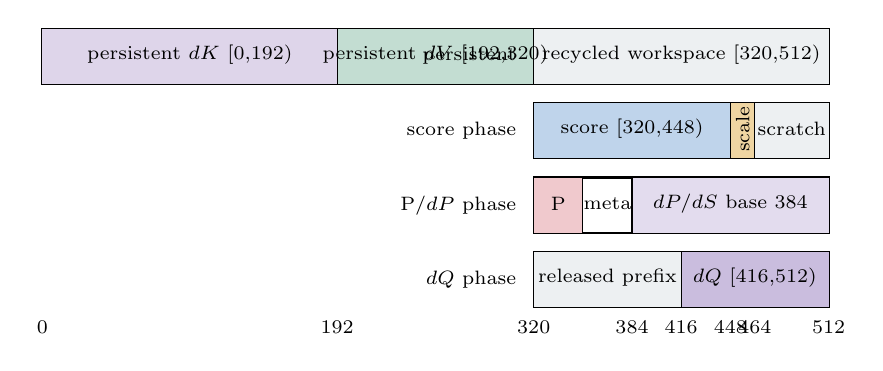
\begin{tikzpicture}[x=0.0195cm,y=.70cm,font=\scriptsize]
  \draw[thick] (0,0) rectangle (512,1);
  \fill[gradientpurple!24] (0,0) rectangle (192,1);
  \fill[outputgreen!28] (192,0) rectangle (320,1);
  \fill[lightgray] (320,0) rectangle (512,1);
  \draw (192,0)--(192,1);
  \draw (320,0)--(320,1);
  \node at (96,.53) {persistent $dK$ [0,192)};
  \node at (256,.53) {persistent $dV$ [192,320)};
  \node at (416,.53) {recycled workspace [320,512)};

  \draw[thick] (320,-1.35) rectangle (512,-.35);
  \fill[scoreblue!30] (320,-1.35) rectangle (448,-.35);
  \fill[scaleyellow!42] (448,-1.35) rectangle (464,-.35);
  \fill[lightgray] (464,-1.35) rectangle (512,-.35);
  \draw (448,-1.35)--(448,-.35);
  \draw (464,-1.35)--(464,-.35);
  \node at (384,-.82) {score [320,448)};
  \node[rotate=90] at (456,-.82) {scale};
  \node at (488,-.82) {scratch};

  \draw[thick] (320,-2.70) rectangle (512,-1.70);
  \fill[probred!28] (320,-2.70) rectangle (352,-1.70);
  \fill[gradientpurple!20] (384,-2.70) rectangle (512,-1.70);
  \draw (352,-2.70)--(352,-1.70);
  \draw (384,-2.70)--(384,-1.70);
  \node at (336,-2.17) {P};
  \node at (368,-2.17) {meta};
  \node at (448,-2.17) {$dP/dS$ base 384};

  \draw[thick] (320,-4.05) rectangle (512,-3.05);
  \fill[lightgray] (320,-4.05) rectangle (416,-3.05);
  \fill[gradientpurple!38] (416,-4.05) rectangle (512,-3.05);
  \draw (416,-4.05)--(416,-3.05);
  \node at (368,-3.52) {released prefix};
  \node at (464,-3.52) {$dQ$ [416,512)};

  \foreach \x in {0,192,320,384,416,448,464,512}
    \node[below] at (\x,-4.12) {\x};
  \node[anchor=east] at (315,.5) {persistent};
  \node[anchor=east] at (315,-.85) {score phase};
  \node[anchor=east] at (315,-2.20) {P/$dP$ phase};
  \node[anchor=east] at (315,-3.55) {$dQ$ phase};
\end{tikzpicture}
\caption{Retained logical TMEM map.  dK spans a 128-column main tile and a
64-column tail; dV spans 128 columns.  The score uses [320,448), its scale page
starts at 448, and the compact dQ accumulator uses [416,512).  P, dP, and dS
reuse retired score/dQ addresses according to phase.}
\label{fig:bwd-tmem-map}
\end{figure}

The most important consequence is negative: another complete M128$\times$N128
FP32 score bank needs 128 columns, but no such bank exists.  Splitting a score
or dQ issue can expose an earlier prefix, yet barriers cannot manufacture
storage.  Experiments that drain half of persistent dV to buy columns lose
more to scratch traffic than they gain from score lookahead.

\subsection{The alias boundary defines legal issue order}

The transient region follows the ownership chain
\begin{equation}
  \text{score}\rightarrow
  \text{P publication}\rightarrow
  dP/dV\ \text{consume}\rightarrow
  dS\rightarrow dQ\ \text{consume}\rightarrow
  \text{next score}.
  \label{eq:bwd-alias-chain}
\end{equation}
The next score cannot overwrite columns 416--447 until the current dQ
consumer has captured that prefix.  Conversely, delaying score issue until
all dQ publication completes exposes unnecessary latency.  The retained
schedule uses issue markers: score and dQ consumers may enqueue their TMEM
loads after the producer instruction has been issued, then let the native
TMEM fence cover completion.  Full completion barriers remain for final
drain and lifetime proof.

\subsection{Shared memory and register boundary}

The profiled hot specialization uses 231,484 bytes of dynamic shared memory,
128 registers per thread, and no local stack or spills.  Shared memory carries
the TMA-fed Q/K/V/$G$ views, Q/dS peer exchange, statistics, and instruction
descriptors.  The kernel is already at the practical register boundary:
an additional score buffer is ruled out by TMEM capacity.  The original
adaptive mixed-dP attempt also aliased its fixed dP scale word with the live
adaptive score scale page, causing repeatable tile-local corruption.  Giving
those values distinct lifetime-safe pages produces a stable 128-register,
zero-spill specialization.  Useful further pipelining still needs a different
ownership topology or an upstream/downstream fusion, not another local barrier
stage.

\subsection{Only dQ is a global reduction}

For an owner $o$, the kernel forms a partial
\begin{equation}
  dQ^{(o)}=\alpha\,dS^{(o)}K^{(o)},\qquad
  dQ=\sum_o dQ^{(o)}.
  \label{eq:dq-owner-reduction}
\end{equation}
The retained implementation publishes these partials with
\code{cp.reduce.async.bulk.tensor} addition.  It is not a scalar atomic loop.
At S8192/H8 the FP32 version moved 830.5 MB into the reduction path, 16.5
times the final 50.3 MB FP32 dQ tensor.  The retained BF16 reduction halves
that payload.  dK and dV stay in TMEM for their complete owner lifetime and
are stored once, so there is no dK/dV atomic mechanism to replace.

\section{Retained Adaptive FP4+FP8 Kernel}

\subsection{End-to-end dataflow}

Algorithm~\ref{alg:retained-bwd} describes one owner iteration.  It is a
dependency description rather than a serialized instruction listing:
independent loader, tensor, statistics, compute, and reducer roles overlap
whenever the lifetime constraints of Figure~\ref{fig:bwd-tmem-map} permit.

\begin{algorithm}[htbp]
\caption{Retained adaptive low-precision backward for one K/V owner}
\label{alg:retained-bwd}
\small
\begin{tabularx}{\textwidth}{@{}r p{.19\textwidth} X@{}}
\toprule
& Owner & Action \\
\midrule
0 & preprocessing & Compute $r=\langle O,G\rangle$ and $L\log_2e$; pack
$2^2G$ and $2^2V$ to E4M3; overlap the BF16 dQ clear. \\
1 & loader & Bring compact adaptive Q/K, V, and $G$ views into their
instruction-facing shared-memory stages. \\
2 & tensor issuer & Issue three K64 NVFP4 score commands into
TMEM [320,448), using the per-head E4M3 scale page. \\
3 & compute warps & Read N32 score fragments, apply saved LSE and causal mask,
and publish $Q_{\mathrm{E4M3}}(2^8\widetilde P)$ directly to TMEM. \\
4 & tensor issuer & Issue E4M3 $dP=GV^\mathsf T$ and
$dV=P^\mathsf TG$ commands into their FP32 accumulators. \\
5 & compute warps & Center scaled dP by $2^4r$, multiply by the represented
P, and emit both E4M3 dS orientations at scale $2^{12}$. \\
6 & tensor issuer & Issue mixed E4M3$\times$E2M1 dK and dQ commands; retain
dK/dV and publish dQ issue markers. \\
7 & reducers & Drain dQ in x32 fragments, apply
$\alpha/(2^{12}m_h)$, and perform BF16 TMA reductions to global memory. \\
8 & owner epilogue & Apply the dK and dV corrections and store each once;
release the persistent owner state. \\
\bottomrule
\end{tabularx}
\end{algorithm}

\subsection{Quantization is fused where the value is born}

The implementation follows one rule: conversion should happen in the producer
that already owns the FP32 or BF16 fragment.  In particular:

\begin{itemize}
  \item $G$, V, row dot products, and LSE conversion share one mandatory
  linear preprocessing pass.
  \item P is converted directly from the score fragment and stored in its
  final E4M3 TMEM orientation.
  \item dS is converted directly from four N32 producer fragments.  The code
  simultaneously forms local-dQ, peer-dQ, and dK-facing layouts.
  \item Q/K projection integration, described in
  Section~\ref{sec:projection-integration}, creates the four E2M1 layouts from
  projection-epilogue registers rather than rereading BF16 Q/K.
\end{itemize}

This is materially different from fake quantization, in which a BF16 tensor
is written to HBM and a separate kernel rereads, quantizes, and transposes it.
The fallback packers remain useful for validation and shallow projection
depths, but they are not the intended integrated dataflow.

\subsection{P reuse joins dV and dS}

The E4M3 P code consumed by dV is also the value used in
Equation~\ref{eq:fused-ds}.  Reusing the exact bits has two benefits.  It
removes a second BF16 P representation, and it ensures that the softmax
derivative is taken with respect to the same represented P used by the dV
tensor product.  The fixed powers satisfy
\begin{equation}
  (2^8P)\,[2^4(dP-r)] = 2^{12}dS,
  \label{eq:scale-factorization}
\end{equation}
so the producer needs packed half arithmetic and one native E4M3 conversion,
not general scale multiplies.

The row term is published as FP16 after being multiplied by $2^4$.  This cuts
the shared loads and registers of the eight native-x32 consumers.  The final
two words of the first P fragment are pre-unpacked into otherwise-unused
registers, shortening the dependent dS loop without extending its live range.

\subsection{Score and dQ use issue-before-completion handoffs}

Score consumers do not first spin on a full completion event.  Once all three
NVFP4 commands are queued, the tensor role publishes \code{score\_issued};
the compute warps enqueue synchronous TMEM reads and rely on
\code{tensor\_load\_wait} for actual data readiness.  The ordinary
\code{score\_done} event stays live for statistics and final drain.

dQ uses the same pattern.  The tensor role publishes \code{dq\_issued} after
the mixed dQ command is queued.  Reducers begin their progressive prefix
loads, allowing columns 416--447 to retire earlier for the following score.
This reduces exposed producer-to-consumer latency without allocating another
TMEM accumulator or weakening the final lifetime proof.

\subsection{BF16 dQ is the projection-ready endpoint}

The default public API preserves an FP32 dQ result: owners reduce into BF16,
then a linear epilogue widens the completed tensor.  When the next learned
linear backward accepts BF16, \code{return\_bf16\_dq=True} omits that pass and
the FP32 allocation.  The represented operation is unchanged; the remaining
difference is the order of nondeterministic owner reductions.

The direct-BF16 endpoint is the retained deployable boundary.  Suppressing dQ
publication entirely measured a lower floor, but a correct consumer cannot
use a partial tile:
\begin{equation}
  dQ_{\mathrm{complete}}[I,:]
  =\sum_o dQ^{(o)}[I,:].
  \label{eq:complete-dq-tile}
\end{equation}
Under K/V ownership, the contributing owners are unclustered.  Removing the
global BF16 reduction requires a q-centric schedule or a larger fused
projection/reduction topology.

\subsection{Current compile-time state}

The result tables use:
\begin{align*}
  \code{TK\_FA4\_BWD\_FP8DPDV\_BF16\_DQ\_REDUCTION} &= 1,\\
  \code{TK\_FA4\_BWD\_FP8DPDV\_TWO\_COMMAND\_SCORE} &= 0,\\
  \code{TK\_FA4\_BWD\_FP8DPDV\_HALF\_DQ\_REDUCTION\_CEILING} &= 0,\\
  \code{TK\_FA4\_BWD\_FP8DPDV\_SKIP\_DQ\_REDUCTION\_CEILING} &= 0,\\
  \code{TK\_FA4\_BWD\_FP8DPDV\_SKIP\_DQ\_WIDEN\_CEILING} &= 0.
\end{align*}
The hot specialization remains at 128 registers with zero spill loads,
zero spill stores, and the exact three-command score.

\section{Learned Projection Integration}
\label{sec:projection-integration}

\subsection{What projection means}

Flatten batch and sequence into $M=BS$, let the model hidden width be $K$,
and concatenate the Q/K/V weights:
\begin{equation}
  W_{QKV}=
  \begin{bmatrix}W_Q\\W_K\\W_V\end{bmatrix},\qquad
  Y_{QKV}=XW_{QKV}^{\mathsf T}=[Q\mid K\mid V].
  \label{eq:qkv-projection}
\end{equation}
This is a learned GEMM with reduction dimension $K$.  It is separate from the
attention score contraction in Equation~\ref{eq:score-contraction-summary},
whose reduction dimension is the head dimension 192.

The previous integration ceiling assumed that an upstream projection could
somehow emit the adaptive E2M1 operands.  The current implementation makes
that producer real: a persistent SM100 NVFP4 GEMM computes
Equation~\ref{eq:qkv-projection} and publishes the forward-native Q/K E2M1
payloads, the backward Q/K views, and transposed MXFP4 V directly from its
output register fragments.  BF16 Q/K/V stores are optional rather than part
of the low-precision contract.  Q and K have per-head depth 192; V has depth
128.  Packed weight rows are ordered as all Q heads, all K heads, then all V
heads.

\subsection{NVFP4 learned-projection equation}

For a 16-value activation block $b=(i,c)$, containing one row and columns
$16c{:}16(c+1)$, the standalone quantizer selects one global dequantizer
$g_X$ and one local E4M3 dequantizer $s^X_{i,c}$.  In simplified notation,
\begin{align}
  g_X &\approx \frac{\lVert X\rVert_\infty}{6\cdot448},\\
  s^X_{i,c} &= Q_{\mathrm{E4M3}}\!\left(
    \frac{\max_{16c\le k<16(c+1)}|X_{ik}|}{6g_X}
  \right),\\
  X^4_{ik} &= Q_{\mathrm{E2M1}}\!\left(
    \frac{X_{ik}}{g_Xs^X_{i,c}}
  \right),\qquad
  \widehat X_{ik}=g_Xs^X_{i,c}X^4_{ik}.
  \label{eq:nvfp4-projection-operand}
\end{align}
Activations retain this $1\times16$ rule because each token row is an
independent sample.

Learned weights instead use a transpose-consistent $16\times16$ rule.  For
$B_{r,c}=\{(j,k):16r\le j<16(r+1),\ 16c\le k<16(c+1)\}$,
\begin{align}
  s^W_{r,c}
    &=Q_{\mathrm{E4M3}}\!\left(
      \frac{\max_{(j,k)\in B_{r,c}}|W_{jk}|}{6g_W}
    \right),\\
  W^4_{jk}
    &=Q_{\mathrm{E2M1}}\!\left(
      \frac{W_{jk}}{g_Ws^W_{r,c}}
    \right),\qquad
  \widehat W_{jk}=g_Ws^W_{r,c}W^4_{jk}.
  \label{eq:nvfp4-projection-weight-2d}
\end{align}
The same local scale is repeated into the sixteen hardware $1\times16$
scale records covered by $B_{r,c}$.  Consequently packing $W^{\mathsf T}$
does not choose a second, incompatible set of scales:
\begin{equation}
  \mathcal Q^{2D}_{\mathrm{NV4}}(W^{\mathsf T})
  =\Pi_{\mathsf T}\!\left(
    \mathcal Q^{2D}_{\mathrm{NV4}}(W)
  \right),
  \label{eq:nvfp4-weight-transpose-consistency}
\end{equation}
where $\Pi_{\mathsf T}$ transposes payload blocks and their scale page.  This
is a representation invariant for forward and dgrad, rather than a claim
that the larger block minimizes one-shot quantization error.

The persistent projection computes
\begin{equation}
  \widehat Y_{ij}
  =\sum_{k=1}^{K}\widehat X_{ik}\widehat W_{jk}
  =g_Xg_W
   \sum_b
   \mma_{\mathrm{E2M1}}\!\left(
     X^4_{i,b},W^4_{j,b};s^X_{i,b},s^W_{j,b}
   \right),
  \label{eq:nvfp4-projection}
\end{equation}
accumulates in FP32 TMEM and multiplies by the two global dequantizers.  The
implementation uses M256$\times$N256 output tiles, K256 reduction steps, a
two-CTA cluster, and a four-stage input ring.  Each output fragment is rounded
once to BF16 before its optional BF16 store and low-precision publication, so
all published views share one rounding point.

\subsection{Pair-native RoPE in the projection epilogue}

The first composed forward/backward evaluation omitted rotary position
embedding and therefore did not represent the Llama attention boundary.  The
unified QKV projection now optionally applies full-head RoPE to Q and K before
either BF16 or low-precision publication.  For $D_{QK}=192$, write the usual
split-half rotary coordinates of one unrotated head as
\begin{equation}
  u=[a_0,\ldots,a_{95},b_0,\ldots,b_{95}]^{\mathsf T},
  \qquad
  \Pi u=[a_0,b_0,a_1,b_1,\ldots,a_{95},b_{95}]^{\mathsf T}.
  \label{eq:rope-pair-permutation}
\end{equation}
The Q and K projection-weight rows are converted once to the $\Pi$ order.
Because $\Pi$ is orthogonal and is common to Q and K,
\begin{equation}
  (\Pi q)^{\mathsf T}(\Pi k)=q^{\mathsf T}k,
  \label{eq:rope-permutation-dot-invariance}
\end{equation}
so this storage choice does not alter the unrotated score operator.  It makes
each rotary plane local to one adjacent BF16 pair in the projection epilogue.

For token $t$ and rotary plane $p$, define
\begin{equation}
  R_{t,p}=
  \begin{bmatrix}
    c_{t,p} & -s_{t,p}\\
    s_{t,p} &  c_{t,p}
  \end{bmatrix},
  \qquad
  \widetilde u_{t,p}=R_{t,p}(\Pi u_t)_p.
  \label{eq:pair-native-rope}
\end{equation}
The epilogue applies Equation~\ref{eq:pair-native-rope} to the rounded Q/K
register fragment and then forms every consumer representation from that
rotated fragment:
\begin{align}
  \widetilde Q_R&=\mathcal R_t(\Pi Q_R),
  &C_Q&=Q_{\mathrm{E2M1}}(m^Q_h\widetilde Q_R),\\
  \widetilde K_R&=\mathcal R_t(\Pi K_R),
  &C_K&=Q_{\mathrm{E2M1}}(m^K_h\widetilde K_R).
  \label{eq:projection-rope-then-quantize}
\end{align}
Consequently the optional BF16 Q/K tensors, forward score operands, and all
backward Q/K byte layouts represent the same rotated operator.  V is not
modified.  The packed implementation evaluates both coordinates with one
BF16x2 multiply and one BF16x2 fused multiply-add; this deliberately accepts
one additional BF16 rounding at the already-BF16 publication boundary rather
than expanding every live pair into FP32 registers.

Attention backward returns derivatives with respect to the rotated tensors.
Before projection dgrad or weight-gradient GEMMs, each Q/K pair is mapped
back to the pair-native projection output by
\begin{equation}
  d(\Pi u_t)_p=R_{t,p}^{\mathsf T}d\widetilde u_{t,p}.
  \label{eq:inverse-rope-gradient}
\end{equation}
The reference implementation applies Equation~\ref{eq:inverse-rope-gradient}
in-place to the Q and K fields of the interleaved BF16
$[dQ\mid dK\mid dV]$ tensor; dV is bit-preserved.  A model may keep Q/K
weights and their optimizer state in pair-native row order.  Export to a
split-half checkpoint requires only the inverse row permutation $\Pi^{\mathsf
T}$.

A projection-dgrad specialization now fuses the same inverse map into its
delayed-scale NVFP4 operand producer.  For a 16-value projection-input block
$b$, it publishes
\begin{equation}
  C^{\nabla,4}_{t,b}
  =Q_{\mathrm{E2M1}}\!\left(
    \frac{\mathcal R_t^{\mathsf T}
      [d\widetilde Q_t\mid d\widetilde K_t\mid dV_t]_b}
         {g_\nabla s^\nabla_{t,b}}
  \right),
  \label{eq:inverse-rope-gradient-nvfp4-handoff}
\end{equation}
where $\mathcal R_t^{\mathsf T}$ acts on Q/K pairs and is the identity on V.
The transform occurs after the attention boundary's BF16 rounding and before
local amax selection, so its E2M1 payload and scale page are bit-exact with
the reference sequence ``inverse RoPE, then NVFP4 quantize.''  An optional
store republishes the inverse-rotated BF16 tile for projection weight-gradient
consumers.  That store preserves the reference bits and is not a performance
penalty in the measured kernel: its asynchronous BF16 publication overlaps
the packing tail.  Both forms are retained, with republication selected when
projection weight-gradient consumers require the inverse-rotated BF16 tile.

\subsection{One Q/K payload shared by forward and backward}

For a BF16-rounded Q register slice $Q_R$ and its head multiplier $m^Q_h$, the
epilogue computes
\begin{equation}
  C_Q=Q_{\mathrm{E2M1}}(m^Q_hQ_R).
  \label{eq:projection-epilogue-q}
\end{equation}
The same codes are rearranged into:
\begin{align}
  \mathcal L_{Q,\mathrm{seq}}(C_Q)
    &\in\mathrm{uint8}^{B\times H\times192\times S},\\
  \mathcal L_{Q,\mathrm{depth}}(C_Q)
    &\in\mathrm{uint8}^{B\times H\times S\times96}.
  \label{eq:q-layout-functions}
\end{align}
For K it independently forms $C_K=Q_{\mathrm{E2M1}}(m^K_hK_R)$ and publishes
\begin{align}
  \mathcal L_{K,\mathrm{aligned}}(C_K)
    &\in\mathrm{uint8}^{B\times S\times H\times192},\\
  \mathcal L_{K,\mathrm{depth}}(C_K)
    &\in\mathrm{uint8}^{B\times H\times S\times96}.
  \label{eq:k-layout-functions}
\end{align}
The compact tensors $\mathcal L_{Q,\mathrm{depth}}$ and
$\mathcal L_{K,\mathrm{depth}}$ are the storage allocation, not copies made
for backward.  Forward obtains typed E2M1 views of the same bytes while
backward consumes uint8 views.  The forward scale hierarchy is
\begin{align}
  s^{Q}_{\mathrm{local}}=s^{K}_{\mathrm{local}}&=448,\\
  g^Q_h&=\frac{1}{448m^Q_h},\qquad
  g^K_h=\frac{1}{448m^K_h},\\
  \widehat Q_R=g^Q_hs^Q_{\mathrm{local}}C_Q&=\frac{C_Q}{m^Q_h},\qquad
  \widehat K_R=g^K_hs^K_{\mathrm{local}}C_K=\frac{C_K}{m^K_h}.
  \label{eq:shared-qk-forward-reconstruction}
\end{align}
Thus forward and backward consume one represented Q/K operator.  There is no
second forward payload and no conversion between the two APIs.

Together with the optional BF16 Q/K store, one register slice can therefore
emit the ordinary tensor and its consumer-specific E2M1 views.
Aligned-U4 rows use eight E2M1 bytes followed by an eight-byte hole for every
16 logical values.  Compact depth rows pack two E2M1 values per byte without
those holes.

The four low-precision tensors are bit-exact against the standalone
precomputed-scale packer.  Fused and separate publication therefore have
identical accuracy; their difference is only movement and scheduling.

\subsection{Single-quantization pure-FP4 Q/K fanout}

The pure-FP4 backward needs two additional compact Q/K operand views for its
block-scaled dQ and dK instructions.  A naive unified producer first formed
the four adaptive forward/backward views above, then quantized the same Q/K
register fragment a second time at the pure route's fixed multiplier.  The
aggressive specialization instead performs one fixed-scale quantization,
\begin{equation}
  C_X^{(16)}=Q_{\mathrm{E2M1}}(16X_R),\qquad X\in\{Q,K\},
  \label{eq:pure-projection-single-quant}
\end{equation}
and fans those codes directly into every consumer layout,
\begin{equation}
  \mathcal B_{QK}^{\mathrm{pure}}
  =\left\{\Pi_\ell\!\left(C_{\chi(\ell)}^{(16)}\right)\right\}_{\ell=1}^{6},
  \qquad \chi(\ell)\in\{Q,K\}.
  \label{eq:pure-projection-layout-fanout}
\end{equation}
Here the six members are the four aligned/compact score and gradient layouts
shared with the ordinary API plus the compact dQ/dK matrix operands.  The
layout maps $\Pi_\ell$ change byte placement only; no member requantizes the
fragment.  The fixed representation also removes the adaptive seven-word
head record from this specialization.  Its forward scale hierarchy is
\begin{equation}
  s^Q_{\mathrm{local}}=s^K_{\mathrm{local}}=448,
  \qquad g^Q=g^K=\frac{1}{448\cdot16},
  \label{eq:pure-projection-forward-scales}
\end{equation}
while the compact backward dQ/dK operands need no materialized scale tensors.
All six payloads and the forward scale pages are bit-exact against the
standalone fixed-scale publisher.  This is an intentionally pure-only
contract: adaptive FP4+FP8 continues to use the robust per-head record.

\subsection{Projection-native MXFP4 V}

For the BF16-rounded projection fragment, define the two-dimensional tile
$T_{u,v}=\{(t,d):32u\le t<32(u+1),\ 32v\le d<32(v+1)\}$.  The retained
MXFP4 policy forms one E8M0 scale for the complete tile,
\begin{align}
  s^V_{u,v}&=Q_{\mathrm{E8M0}}\!\left(
    \frac{\max_{(t,d)\in T_{u,v}}|V_{R,t,d}|}{6}
  \right),\\
  C^V_{t,d}&=Q_{\mathrm{E2M1}}\!\left(
    \frac{V_{R,t,d}}{s^V_{u,v}}
  \right),\qquad
  \widehat V_{t,d}=s^V_{u,v}C^V_{t,d}.
  \label{eq:projection-native-v}
\end{align}
The scale is repeated into the thirty-two hardware $1\times32$ scale records
inside $T_{u,v}$.  The same codes and scale are then written in both the
feature-major layout required by forward PV and the row-major layout required
by backward dP.  Therefore
\begin{equation}
  \mathcal B^{V}_{\mathrm{bwd}}
  =\Pi_{SD}\!\left(\mathcal B^{V}_{\mathrm{fwd}}\right),
  \label{eq:mxfp4-v-transpose-consistency}
\end{equation}
with no independent row-scale selection after the transpose.  This removes
the BF16 V reread and standalone row-to-column packing from forward setup and
makes the two MXFP4 consumers observe one represented V operator.  The legacy
$1\times32$ policy remains available only as an explicit diagnostic.

The complete optional publication contract is
\begin{equation}
  \mathcal B_{QKV}=
  \left\{
    C_Q,C_K,s^Q,g^Q,s^K,g^K,C^V,s^V,
    \mathcal L_{Q,\mathrm{seq}},\mathcal L_{K,\mathrm{aligned}},
    m^Q_h,m^K_h
  \right\}
  \cup
  \left\{Q_{\mathrm{BF16}},K_{\mathrm{BF16}},V_{\mathrm{BF16}}\right\}_{\mathrm{optional}}.
  \label{eq:unified-qkv-bundle}
\end{equation}
When every downstream consumer accepts $\mathcal B_{QKV}$, disabling the
three BF16 stores avoids $BSH(192+192+128)\cdot2=BSH\cdot1024$ bytes of
global publication.

\subsection{Scale ownership at the composed D64 boundary}

The projection epilogue also publishes E4M3 Q, K, and V for attention
backward.  These are deliberately independent of the forward FP4 multipliers
$m^Q_h$ and $m^K_h$.  Let $\lambda=2^2=4$ be the fixed E4M3 publication
factor and let $G=dO$ denote the loss-scaled upstream gradient.  Backward
consumes
\begin{equation}
  Q'=\lambda Q,\qquad K'=\lambda K,\qquad
  V'=\lambda V,\qquad G'=\lambda G,
  \label{eq:d64-fixed-fp8-publication}
\end{equation}
and compensates the score product with
\begin{equation}
  \alpha'=\frac{\alpha}{\lambda^2}=\frac{\alpha}{16}.
  \label{eq:d64-fixed-fp8-score-scale}
\end{equation}
The represented softmax is consequently unchanged.  Applying the chain rule
in encoded units gives
\begin{equation}
  dV'=\lambda dV,\qquad dP'=\lambda^2dP,\qquad
  dQ'=\lambda dQ,\qquad dK'=\lambda dK.
  \label{eq:d64-fixed-fp8-gradient-units}
\end{equation}
If dynamic loss scaling contributes $L$, inverse RoPE and the QKV projection
consume each attention-gradient field with $1/(\lambda L)$.  Optional
calibration gains $c_Q,c_K,c_V$ remain field-local,
\begin{equation}
  \bar dQ=\frac{c_Q}{\lambda L}R^{\mathsf T}dQ',\qquad
  \bar dK=\frac{c_K}{\lambda L}R^{\mathsf T}dK',\qquad
  \bar dV=\frac{c_V}{\lambda L}dV'.
  \label{eq:d64-field-local-gradient-decode}
\end{equation}
The default is $c_Q=c_K=c_V=1$.  A forward probability approximation does
not implicitly own these gains: any non-unit correction must be exported by
the topology and validated per field.  In particular, a historical common
0.632 multiplier is not inferred from the softmax mode because it suppresses
Q/K/V gradient norms without changing the output-projection weight gradient.

\subsection{Adaptive scale production remains a contract}

Outside the fixed-scale pure specialization, the fused epilogue
\emph{consumes} the seven-word per-head scale record; it does not calculate
Equation~\ref{eq:head-stats} from its distributed output tiles.  A true
same-launch amax/RMS reduction would need cross-CTA completion before earlier
Q/K tiles could be finalized, defeating the simple streaming epilogue.

The current API consequently exposes three legal scale sources:

\begin{enumerate}
  \item the standalone robust Q/K reduction, used for validation;
  \item precomputed device-resident scales from an upstream producer or
  calibration policy;
  \item a future learned-projection epilogue with a delayed, pipelined, or
  model-defined scale contract.
\end{enumerate}

Current projection validation derives the record from BF16 reference Q/K
before timing the projection hot stage.  The measured epilogue is real, but
this detail prevents interpreting its timing as a solved same-step adaptive
scale reduction.  An integrated model must state how $m^Q_h$ and $m^K_h$ are
supplied.

\subsection{Upstream low-precision dO contract}

The backward also needs two MXFP4 orientations of the output gradient
$G=dO$ and the softmax centering term.  For row blocks $b_r$ and transposed
column blocks $b_c$, the producer emits
\begin{align}
  C^{G,r}_{i,b_r}&=Q_{\mathrm{E2M1}}
    \!\left(G_{i,b_r}/s^{G,r}_{i,b_r}\right),\\
  C^{G,c}_{d,b_c}&=Q_{\mathrm{E2M1}}
    \!\left(G^{\mathsf T}_{d,b_c}/s^{G,c}_{d,b_c}\right),\\
  \delta_i&=\sum_{d=1}^{128}O_{i,d}G_{i,d}.
  \label{eq:upstream-dout-contract}
\end{align}
One fused producer reads dO once and publishes both code/scale orientations
and $\delta$.  This is the upstream boundary used by the all-MX experiments;
the separate row quantizer, column quantizer, and delta kernel remain only as
a bit-exact diagnostic reference.

\subsection{Probability replay boundary}

Within one backward iteration, the retained route reuses the represented
E4M3 probability produced for dV when forming dS rather than reevaluating the
exponential.  If $C^P$ denotes that code,
\begin{equation}
  \widehat{dS}_{ij}=\widehat P_{ij}
    \left(\widehat{dP}_{ij}-\delta_i\right),\qquad
  \widehat P_{ij}=s^P_{ij}C^P_{ij}.
  \label{eq:represented-p-replay}
\end{equation}
This is a local register/TMEM reuse contract, not an HBM cache.  Caching a
complete MXFP4 probability matrix across forward and backward would require
\begin{equation}
  M_P=\frac{BHS^2}{2}
      +BH\left(\frac{S}{128}\right)^2(32\cdot16)
      \quad\text{bytes}
  \label{eq:probability-cache-bytes}
\end{equation}
for payload plus scale pages.  At S8192/H8 this is approximately 272 MiB, so
the write/read traffic overwhelms the measured local replay saving.

\subsection{Reduction-width dispatch}

Publication cost is controlled by projection reduction depth $K$, not by head
count in isolation.  With only four K256 steps at K1024, one consumer
warpgroup cannot hide BF16 rounding, E2M1 conversion, transpose, and four
global layouts behind the tensor producer.  The separate 32-register packer
spreads that work over a wider CTA grid.  With twelve or more K256 steps,
publication hides under the MMA pipeline and avoiding the BF16 HBM reread is
decisive.

The legacy Q/K-only public dispatcher therefore selects
\begin{equation}
  \operatorname{publish}(K)=
  \begin{cases}
    \text{NVFP4 projection + parallel packer},&K<3072,\\
    \text{fused register-epilogue publication},&K\ge3072.
  \end{cases}
  \label{eq:projection-dispatch}
\end{equation}
Both paths return one \code{B300AdaptiveLowpOperands} object and identical
layout bits.

The unified QKV entry point always uses the fused projection epilogue because
V publication and optional BF16 suppression are part of the single producer
contract.  Its projection scratch aliases the Q/K code staging region with
the V BF16-pair staging region: they are disjoint in lifetime.  This reduces
static scratch from 10,704 to 8,592 bytes without changing the hot backward
kernel.

\subsection{Projection backward}

For the PyTorch weight convention in Equation~\ref{eq:learned-projections-summary},
the input-gradient contribution is
\begin{equation}
  dX=dQW_Q+dKW_K+dVW_V.
  \label{eq:projection-dgrad}
\end{equation}
The first integration writes fully reduced BF16 gradients into one per-head
buffer ordered as $[dQ_{192},dK_{192},dV_{128}]$.  A persistent weight packing
step stores $[W_Q,W_K,W_V]$ in the matching order.  One, two, or four
head-contiguous GEMMs consume the buffer, selected by shape, without three
standalone gradient tensors or an explicit concatenation.

The newer dQ path joins readiness to the projection reduction loop.  Let
$r$ index a 256-row projection tile, $h$ a head, and $o$ a causal K/V-owner
cluster.  Each of the two CTAs in owner $o$ publishes one release increment
only after all four reducer warps have retired their BF16 TMA reductions and
ordered the async proxy:
\begin{align}
  a_{h,t} &\leftarrow a_{h,t}+1,\qquad
  \mathrm{ready}(h,t,r)\iff a_{h,t}\ge 2(r+1),\\
  t&\in\{2r,2r+1\}.
  \label{eq:dq-head-arrival}
\end{align}
The factor $2(r+1)$ is the exact number of contributing CTAs for either
128-row half of causal row pair $r$.  A device-scope acquire poll is placed
immediately before the first K64 slice of each head, not before the complete
projection tile.  The projection accumulator therefore evaluates
\begin{equation}
  dX_{R,C}=\sum_{h=0}^{H-1}\sum_{j=0}^{2}
    dQ_{R,h,64j:64(j+1)}
    W_{Q,C,h,64j:64(j+1)}^{\mathsf T},
  \label{eq:head-pipelined-dq-projection}
\end{equation}
waiting for head $h$ only when its first $j=0$ slice reaches the load
producer.  This is a reduction-topology integration: readiness is part of the
K loop, rather than a whole-row gate in front of GEMM.

Two FP32 TMEM accumulators alternate output tiles.  While the epilogue drains
slot $p$ to BF16, the tensor warpgroup issues the next output into slot
$p\oplus1$.  This removes the former MMA--epilogue serialization without
allocating TMEM inside the attention kernel; the projection kernel owns all
512 of its own TMEM columns.  The consumer remains at 80 registers with zero
spills, and the attention specialization remains at 128 registers with zero
spills.

A bounded early grid is necessary so projection does not displace the
attention owner grid.  For wide outputs, that bounded grid cannot expand when
attention retires, so an experimental split computes a ready row prefix with
the persistent consumer and a disjoint suffix with the vendor GEMM:
\begin{equation}
  dX=\begin{bmatrix}
    \mathcal P_{\theta}(dQ_{0:R},W_Q)\\
    \mathrm{GEMM}(dQ_{R:S},W_Q)
  \end{bmatrix}.
  \label{eq:dq-projection-tail-split}
\end{equation}
The two streams write disjoint rows.  At S8192/H8 the all-persistent route now
slightly beats attention plus cuBLAS.  H16/H24/H64 still favor the ordinary
BF16 reduction followed by the vendor GEMM, so the public entry point
shape-dispatches to that non-regressing fallback unless the pipelined route is
explicitly forced for profiling.

\subsection{Absorbing a hierarchical dQ sum}

The next experiment removes the \emph{completed} standalone dQ tensor from
the projection contract.  Partition K/V owners by parity and define two BF16
reduction lanes
\begin{equation}
  dQ^{(\ell)}=\sum_{o:\,o\bmod2=\ell}dQ^{(o)},\qquad
  dQ=dQ^{(0)}+dQ^{(1)}.
  \label{eq:dq-two-lane-hierarchy}
\end{equation}
The attention reducer publishes each owner into its compile-time-selected
lane.  Projection then exploits linearity:
\begin{align}
  dX_Q
    &=\left(dQ^{(0)}+dQ^{(1)}\right)W_Q\\
    &=dQ^{(0)}W_Q+dQ^{(1)}W_Q.
  \label{eq:dq-hierarchy-projection}
\end{align}
Both lane products accumulate into the same FP32 TMEM output.  No kernel ever
constructs or consumes a global BF16 array equal to $dQ$.  The ordinary
one-lane producer is a separate template instantiation, so hierarchy indexing
does not add a modulo or branch to the retained path.

The construction is numerically sound but does not improve time.  At
S8192/H8, attention plus cuBLAS measured 0.773824~ms and the two-lane consumer
0.805888~ms, a 32.064~$\mu$s loss, with dX cosine 0.99999422.  At S4096/H24,
the corresponding times were 0.736000~ms and 1.063392~ms, a
327.392~$\mu$s loss, with cosine 0.99999648.  Both projection specializations
compile at 80 registers, two barriers, and zero spills.

Equation~\ref{eq:dq-hierarchy-projection} duplicates the complete weight MMA.
A second implementation instead formed $dQ^{(0)}+dQ^{(1)}$ in shared memory
before one MMA.  Scalar and packed-BF16 serial folds took approximately 2.68
and 2.33~ms.  Moving the fold to idle producer warps and using explicit
128-bit shared transfers improved it to 0.860608~ms at S8192/H8, but remained
slower than the two-MMA form.  The tensor-native hierarchy is therefore kept
only as an opt-in structural diagnostic.

This distinction matters: the experiment eliminates a completed BF16 dQ
\emph{tensor}, but not BF16 global partial traffic.  The producer still emits
the same number of values, split across two arrays, and projection pays either
an additional weight product or an explicit fold.  A winning hierarchy must
also change the pre-publication representation:
\begin{equation}
  \text{owner partials}
  \xrightarrow{\text{on-chip grouping or compact FP8/FP4}}
  \text{projection reduction}.
  \label{eq:dq-winning-hierarchy-contract}
\end{equation}
A winning path performs Equation~\ref{eq:dq-winning-hierarchy-contract}
without a BF16 dQ round trip.  An on-chip super-owner can reduce several K/V
owners before one global write.
Alternatively, compact low-precision partials can make repeated projection
products proportional to the higher FP8/FP4 tensor rate.  Reversing the whole
kernel to q-centric ownership completes dQ locally but transfers the global
reduction to the combined 320 dK/dV features rather than the 192 dQ features,
so it is not the preferred next topology.

\subsection{Stacked low-precision QKV-gradient handoff}

The final experiment combines the three projection-gradient fields before one
NVFP4 projection.  Let $R_t^{\mathsf T}$ apply inverse RoPE to one Q or K
head at token $t$.  For the two-lane diagnostic, the row presented to the
quantizer is
\begin{equation}
  G_t^{(2)}=
  \left[
    R_t^{\mathsf T}\!\left(dQ_t^{(0)}+dQ_t^{(1)}\right)
    \;\middle|\;
    R_t^{\mathsf T}dK_t
    \;\middle|\;
    dV_t
  \right].
  \label{eq:stacked-qkv-gradient-row}
\end{equation}
The producer loads a K128 tile, assigns its two K64 halves to independent row
groups, performs the dQ lane addition and inverse rotations in registers, and
chooses one delayed-scale NVFP4 representation per K16 block:
\begin{align}
  s^G_{t,b}
    &=Q_{\mathrm{E4M3}}\!\left(
      \frac{\max_{k\in b}|G^{(2)}_{t,k}|}{6\bar g_G}
    \right),\\
  C^G_{t,k}
    &=Q_{\mathrm{E2M1}}\!\left(
      \frac{G^{(2)}_{t,k}}{\bar g_Gs^G_{t,b}}
    \right),\qquad
  \widehat G_{t,k}=\bar g_Gs^G_{t,b}C^G_{t,k}.
  \label{eq:stacked-qkv-gradient-nvfp4}
\end{align}
With the correspondingly stacked persistent weight
$W_\Sigma=[W_Q^{\mathsf T},W_K^{\mathsf T},W_V^{\mathsf T}]^{\mathsf T}$,
one projection computes
\begin{equation}
  \widehat{dX}_{t,j}
  =\bar g_Gg_W\sum_b
    \mma_{\mathrm{E2M1}}\!\left(
      C^G_{t,b},C^W_{j,b};s^G_{t,b},s^W_{j,b}
    \right).
  \label{eq:stacked-qkv-gradient-projection}
\end{equation}
This form avoids a completed dQ array, but enabling per-tile readiness changes
the attention schedule.  Even a one-lane signaling control slows the attention
kernel.  The retained activation-only variant therefore uses the ordinary
unsignaled BF16 dQ endpoint and replaces $dQ^{(0)}+dQ^{(1)}$ in
Equation~\ref{eq:stacked-qkv-gradient-row} by completed $dQ$.  It still fuses
inverse RoPE, three-field layout conversion, local scaling, and packing before
the single NVFP4 projection.  It does \emph{not} remove BF16 dQ
materialization, and it does not provide the BF16 QKV tensor required by the
projection weight-gradient GEMM.  The two contracts are therefore reported
separately rather than treating the activation-only result as a complete
training step.

\subsection{Compact NVFP4 dQ handoff}

A second implementation changes the representation at the final
attention--projection boundary without changing the owner reduction.  Let
$D=dQ_{\mathrm{complete}}$ be the private BF16 reduction scratch and let
$\bar g_D$ be a device-resident NVFP4 decode scale supplied by calibration or
a previous step.  For each K16 block $b$, the producer forms
\begin{align}
  s^D_{i,b}
    &=Q_{\mathrm{E4M3}}\!\left(
      \frac{\max_{k\in b}|D_{ik}|}{6\bar g_D}
    \right),\\
  C^D_{ik}
    &=Q_{\mathrm{E2M1}}\!\left(
      \frac{D_{ik}}{\bar g_Ds^D_{i,b}}
    \right),
  \qquad
  \widehat D_{ik}=\bar g_Ds^D_{i,b}C^D_{ik}.
  \label{eq:compact-dq-nvfp4}
\end{align}
The matrix-wide amax pass is absent from this hot path.  With a persistently
packed projection weight
$\widehat W_{jk}=g_Ws^W_{j,b}C^W_{jk}$, the consumer evaluates
\begin{equation}
  \widehat{dX}_{Q,ij}
  =\bar g_Dg_W\sum_b
    \mma_{\mathrm{E2M1}}\!\left(
      C^D_{i,b},C^W_{j,b};s^D_{i,b},s^W_{j,b}
    \right).
  \label{eq:compact-dq-nvfp4-projection}
\end{equation}
The public result contains $\widehat{dX}_Q$, dK, and dV; standalone dQ is not
returned.  The generic NVFP4 consumer uses M256$\times$N256 output tiles,
K256 reduction steps, a two-CTA cluster, FP32 TMEM accumulation, and one BF16
output rounding.  It compiles at 86 registers with two barriers and no spills.

This is a compact \emph{final-tile} handoff, not yet a compact owner-partial
reduction.  The unclustered attention owners still require an additive BF16
TMA target, so $D$ exists as private scratch until the last owner completes:
\begin{equation}
  \{dQ^{(o)}\}_o
  \xrightarrow{\mathrm{BF16\ TMA\ reduction}}
  D
  \xrightarrow{Q_{\mathrm{NV4}}}
  (C^D,s^D,\bar g_D)
  \xrightarrow{\mathrm{NV4\ projection}}
  \widehat{dX}_Q.
  \label{eq:compact-dq-current-boundary}
\end{equation}
It nevertheless measures whether compact projection consumption can repay its
conversion.  Delayed scale overestimates from $1\times$ through $8\times$ the
same-step ideal preserve approximately 0.99098 cosine because the local K16
scales renormalize the blocks.  Underestimates clip: $0.5\times$, $0.25\times$,
and $0.125\times$ give approximately 0.9905, 0.9849, and 0.9637 cosine.
Consequently a conservative delayed policy is viable; a winning fused owner
scheme must still publish tile-ready codes or quantize inside a super-owner.

\subsection{The new ceiling}

Unified projection publication removes three previously exposed costs:
\begin{equation}
  \text{BF16 Q/K/V HBM publication}
  \rightarrow
  \text{Q/K/V HBM reread}
  \rightarrow
  \text{standalone pack/transpose/quantize}.
  \label{eq:removed-qk-roundtrip}
\end{equation}
It does not remove the global dQ reduction.  A timing-only attention run that
suppressed dQ publication reached approximately 0.693 ms at S8192/H8, versus
0.746 ms for the direct-BF16 endpoint.  The head-pipelined route now
participates in readiness and reduction scheduling, but still reads the
globally materialized BF16 sum.  Reaching the remaining floor requires
projection backward to absorb the hierarchical sum before that publication,
not merely observe it earlier.  The two-lane experiment shows more precisely
that absorbing only the \emph{last addition} is also insufficient: owner
grouping or compact publication must remove the BF16 producer traffic at the
same time.

\section{Performance and Accuracy}

\subsection{Measurement boundary}

All headline backward rows are causal B1 with $D_{QK}=192$ and $D_V=128$ on
GPU 0.  The copied BF16 V382 mode and low-precision mode run through the same
extension and scheduler family.  Table~\ref{tab:direct-bf16-results} uses five
warmups and 21 rotated CUDA-event samples with seed 2026081201.  Operand
preparation is outside the standalone backward timing; projection tables state
explicitly whether BF16-to-NVFP4 activation preparation is charged.

These are implementation medians, not peak-throughput estimates.  The result
does not include an optimizer step, projection weight-gradient GEMM, or full
training iteration.

\subsection{Standalone backward}

Reducing dQ in BF16 and returning it directly gives the strongest deployable
backward endpoint:

\begin{table}[htbp]
\centering
\caption{Retained adaptive backward versus the copied BF16 control.  Lower is
better.}
\label{tab:direct-bf16-results}
\small
\begin{tabular}{rrr r r}
\toprule
S & H & BF16 control (ms) & adaptive BF16 dQ (ms) & improvement \\
\midrule
4096  & 24 & 0.704480 & 0.624832 & 11.31\% \\
8192  & 8  & 0.868864 & 0.746432 & 14.09\% \\
8192  & 24 & 2.207200 & 1.888768 & 14.43\% \\
8192  & 64 & 5.560512 & 4.761888 & 14.36\% \\
16384 & 24 & 7.743616 & 6.471232 & 16.43\% \\
16384 & 64 & 20.273727 & 17.068480 & 15.81\% \\
\bottomrule
\end{tabular}
\end{table}

The FP32-return API uses the same BF16 reduction and adds one widening pass.
Skipping that pass saves 2.0--5.0\% relative to the FP32-return adaptive route.
Changing the reduction payload itself from FP32 to BF16 accounts for another
0.5--5.2\%, with the benefit increasing at long sequence.

\subsection{Calibrated and outlier accuracy}

Table~\ref{tab:direct-bf16-quality} compares direct BF16 outputs to the copied
BF16 control.  Values are component cosine, not an aggregate dominated by dV.

\begin{table}[htbp]
\centering
\caption{Calibrated component cosine for the direct-BF16 endpoint.}
\label{tab:direct-bf16-quality}
\small
\begin{tabular}{rr rrr}
\toprule
S & H & dQ & dK & dV \\
\midrule
4096  & 24 & 0.991447 & 0.991379 & 0.999356 \\
8192  & 8  & 0.991533 & 0.991557 & 0.999378 \\
8192  & 24 & 0.991435 & 0.991484 & 0.999360 \\
8192  & 64 & 0.991478 & 0.991487 & 0.999354 \\
16384 & 24 & 0.991560 & 0.991526 & 0.999355 \\
16384 & 64 & 0.991447 & 0.991452 & 0.999345 \\
\bottomrule
\end{tabular}
\end{table}

The robust scale rule in Equation~\ref{eq:robust-clip} matters outside the
calibration distribution.  On a one-percent sparse Q/K outlier test:

\begin{table}[htbp]
\centering
\caption{Sparse-outlier accuracy of the retained adaptive route.}
\label{tab:outlier-quality}
\small
\begin{tabular}{rr rrr}
\toprule
S & H & dQ cosine & dK cosine & dV cosine \\
\midrule
4096 & 24 & 0.962695 & 0.962139 & 0.999070 \\
8192 & 8  & 0.961676 & 0.963121 & 0.998915 \\
\bottomrule
\end{tabular}
\end{table}

The earlier global-amax adaptive rule reached only about 0.753/0.757 dQ/dK
cosine at S4096/H24.  The robust per-head rule improves the outlier regime
without changing the three score instructions, TMEM map, or calibrated result.
It still clips information and is not a proof of training convergence.

\subsection{Learned projection publication}

Table~\ref{tab:projection-charged} charges the current standalone conversion
of BF16 X into the NVFP4 activation operand.  NVFP4 weights are treated as
persistent and prepared once.  The low-precision column uses the automatic
publication policy in Equation~\ref{eq:projection-dispatch}.

\begin{table}[htbp]
\centering
\caption{Q/K learned-projection plus backward-layout production.  The
BF16-input column includes current activation preparation.}
\label{tab:projection-charged}
\small
\begin{tabular}{l rrr}
\toprule
Shape & BF16 GEMM + pack (ms) & BF16 input to NVFP4 auto (ms) & speedup \\
\midrule
S8192/H8/K1024  & 0.163712 & 0.142768 & 1.147$\times$ \\
S4096/H24/K3072 & 0.326704 & 0.206096 & 1.585$\times$ \\
S4096/H64/K8192 & 1.553184 & 0.515616 & 3.012$\times$ \\
\bottomrule
\end{tabular}
\end{table}

If X already arrives in NVFP4, the corresponding hot-stage speedups are
1.473$\times$, 1.933$\times$, and 3.342$\times$.  Q/K cosine against the
BF16 learned projection is approximately 0.99097--0.99098.  Fused versus
separate E2M1 publication is bit-exact.

The dispatcher removes the shallow-K epilogue regression:

\begin{table}[htbp]
\centering
\caption{Automatic projection publication versus forcing the other route.}
\label{tab:projection-dispatch-results}
\small
\begin{tabular}{l l rrr}
\toprule
Shape & auto route & auto (ms) & forced other (ms) & advantage \\
\midrule
S8192/H8/K1024  & separate & 0.111024 & 0.122368 & 1.102$\times$ \\
S4096/H24/K3072 & fused    & 0.169984 & 0.181712 & 1.069$\times$ \\
S4096/H64/K8192 & fused    & 0.462560 & 0.626592 & 1.355$\times$ \\
\bottomrule
\end{tabular}
\end{table}

The dominant gain is real NVFP4 tensor work and reduced A/B traffic.  At deep
K, the fused epilogue adds a movement win by avoiding the BF16 Q/K reread and
standalone transpose.  At K1024, the wider parallel packer is faster than
placing all publication on the persistent GEMM's one consumer warpgroup.
These two tables describe the legacy Q/K-only API.

The unified QKV producer adds projection-native MXFP4 V and allows all three
BF16 stores to be suppressed.  Table~\ref{tab:unified-qkv-projection} compares
it with three BF16 GEMMs followed by the standalone Q/K packer.  Input and
weight NVFP4 operands are already resident in all columns so that the table
isolates projection and publication policy.

\begin{table}[htbp]
\centering
\caption{Unified QKV projection and native forward/backward publication.}
\label{tab:unified-qkv-projection}
\small
\begin{tabular}{l rrr rr}
\toprule
Shape & BF16 + QK pack & unified + BF16 & speedup & unified no BF16 & speedup \\
 & (ms) & (ms) & & (ms) & \\
\midrule
S2048/H8/K1024   & 0.149264 & 0.088688 & 1.683$\times$ & 0.077440 & 1.927$\times$ \\
S4096/H24/K4096  & 0.463744 & 0.328816 & 1.410$\times$ & 0.289552 & 1.602$\times$ \\
\bottomrule
\end{tabular}
\end{table}

Projection Q/K/V cosine is 0.99096--0.99098.  Consuming the native operands
in causal forward gives output cosine 0.990722 at S2048/H8 and 0.991317 at
S4096/H24.  All four backward Q/K layouts are bit-exact against their
standalone publishers.  Under the retained 2-D policy, the forward- and
backward-oriented V payloads are exact transposes and their repeated scale
pages select the same $32\times32$ tile scale.  The legacy standalone V
publishers select independent $1\times32$ scales, so they are intentionally
no longer a byte-level reference.  The forward Q/K tensors and backward
compact tensors alias the same allocation.

The storage reduction is material at long sequence.  Sharing the compact Q/K
payload avoids $BHS\cdot192$ bytes: 12 MiB at S8192/H8 and 18 MiB at
S4096/H24.  Suppressing BF16 Q/K/V publication avoids a further 64 MiB and
96 MiB respectively.  The projection producer also reduces its static shared
scratch by 2,112 bytes, from 10,704 to 8,592 bytes.  This scratch saving does
not change the already near-full shared-memory allocation of the backward
kernel.

\subsection{Two-dimensional scale-contract audit}

The composed D64 path was re-audited with the representation rules in
Equations~\ref{eq:nvfp4-projection-weight-2d} and
\ref{eq:projection-native-v}.  Packing a synthetic weight and independently
packing its transpose produces exactly the transposed E2M1 codes, matching
E4M3 local scales, and the same global scale under the $16\times16$ policy.
The $1\times16$ policy does not provide that invariant.

Sharing scales over two dimensions is stricter and therefore slightly less
accurate for a single isolated tensor.  On the fixed D64 projection audit,
learned-projection cosine changes from 0.990916 with $1\times16$ weights to
0.989259 with $16\times16$ weights; relative L2 changes from 0.13483 to
0.14630.  Decoded V cosine changes from 0.993560 with independently selected
$1\times32$ row/column scales to 0.993031 with one $32\times32$ scale;
relative L2 changes from 0.11332 to 0.11789.  The retained reason for the
two-dimensional policy is not a better one-shot cosine: it is transpose
consistency when fprop and bprop actually consume the two orientations of the
same low-precision representation.  That benefit is only partially active in
the selected hybrid.  Output projection does consume both orientations, but
QKV projection dgrad remains BF16 and attention backward consumes FP8 V.
Consequently, applying one 2-D switch to every learned weight and to V also
charges coarser forward quantization where no transposed FP4 consumer reuses
it.  The policy remains useful for the all-FP4 ladder; the hybrid requires
separate QKV/output-weight switches rather than a blanket 2-D default.

The E8M0 exponent selector must likewise follow the scale geometry.  On the
fixed causal-V activation audit, the $1\times32$ policy minimizes attention
relative L2 at 0.11409 when it rounds up at normalized amax 1.20; ordinary
nearest-power rounding (the 1.50 midpoint) gives 0.12818.  For a shared
$32\times32$ tile the ordering reverses: nearest-power rounding gives 0.12439,
versus 0.12745 with the 1.20 rule.  The retained publisher therefore uses a
BF16-exact 1.203125 cutoff for $1\times32$ and ties-to-even nearest-power
rounding for $32\times32$.  A staged binary matched the independent payload
and scale emulator bit-for-bit for both geometries, with and without causal
interleaving, and passed the unified projection-layout validator.  These are
one-activation representation checks, not convergence measurements.  In the
matched sixteen-layer diagnostic, the new selector improves first-layer
attention-branch relative L2 from 0.37686 to 0.37438, but the final sampled
logit changes are mixed and negligible: cosine changes from 0.68707 to
0.68597 while relative L2 changes from 0.79662 to 0.79494.  Selector rounding
therefore does not explain the much larger optimization-proxy regression.

The implementation cost is below whole-step measurement noise.  In matched
16-layer S4096/H32 GQA runs, the low-precision step measured 76.929~ms with
legacy one-dimensional scales and 76.931~ms with two-dimensional scales.  The
two-dimensional run used independent Q/K FP4 multipliers 2.25 and 2.0 and
unit field gains.  Against an 83.304-ms BF16 step in that run, it measured
1.083$\times$ end-to-end speedup.  This short synthetic-token comparison is a
systems measurement; its 16-layer sampled-logit cosine of 0.6989 is not a
convergence result.

The backward scale audit also found and removed a stale common gain.  The
previous MXFP4-PV comparison silently inferred 0.632 from its forward softmax
mode, yielding initial Q/K weight-gradient norm ratios near 0.593 and a V
ratio near 0.425.  With Equation~\ref{eq:d64-field-local-gradient-decode} and
unit gains, the corresponding Q/K/V ratios are approximately
0.954/0.937/0.961.  Directional error remains after sixteen approximate
layers, however, and norm parity does not imply a more accurate gradient.  If
$r=\lVert\widehat g\rVert/\lVert g\rVert$ and $c$ is the cosine to the BF16
gradient, applying gain $a$ gives
\begin{equation}
  \frac{\lVert a\widehat g-g\rVert_2}{\lVert g\rVert_2}
  = \sqrt{1+(ar)^2-2arc}.
  \label{eq:gain-direction-error}
\end{equation}
For $c\approx0.3$, forcing $ar\approx1$ raises relative error to about 1.18.
Thus the unit-gain endpoint removed a norm confound but amplified a poorly
aligned direction.  It is an audit point, not a calibrated training policy.
The optional NVFP4 QKV-dgrad consumer now folds the same three decode factors
into its E4M3 metadata.  It restores the expected norms but is not selected:
its measured backward is 46.11~ms versus 43.89~ms for the BF16 projection
dgrad route.

No random Hadamard transform or stochastic rounding is charged in the
selected route.  Forward activations use $1\times16$ RNE, learned weights use
$16\times16$ RNE, and QKV projection dgrad plus both weight-gradient GEMMs
remain BF16.  RHT/SR becomes relevant only if those gradient operands are
actually retained in FP4; adding it around the slower diagnostic NVFP4 dgrad
would be fake quantization overhead rather than a numerical fix for the
winner.

A controlled 24-round comparison then put both PV routes on this corrected
contract.  Table~\ref{tab:d64-2d-route-comparison} reports medians for the
synthetic 16-layer S4096 Llama-1.2B training proxy.

\begin{table}[htbp]
\centering
\caption{End-to-end D64 route comparison with 2-D learned weights, 2-D MXFP4
V, independent Q/K multipliers, and unit Q/K/V backward gains.}
\label{tab:d64-2d-route-comparison}
\small
\begin{tabular}{l rrr r r}
\toprule
Route & forward & backward & optimizer & step & speedup \\
 & (ms) & (ms) & (ms) & (ms) & vs BF16 \\
\midrule
BF16 CuTE                 & 27.718 & 45.596 & 10.726 & 84.050 & 1.000$\times$ \\
NVFP4 QK + MXFP4 PV       & 22.466 & 44.239 & 10.732 & 77.428 & 1.086$\times$ \\
NVFP4 QK + exact FP8 PV   & 24.884 & 44.233 & 10.733 & 79.860 & 1.052$\times$ \\
\bottomrule
\end{tabular}
\end{table}

The two low-precision backward times are indistinguishable at this scale; the
MXFP4 route's additional 2.43-ms whole-step gain comes from forward PV.  The
corresponding sampled-logit cosines are 0.69348 for MXFP4 PV and 0.77821 for
exact FP8 PV.  Q/K/V first-layer weight-gradient cosine is
0.27691/0.32003/0.39347 for MXFP4 and
0.44378/0.45383/0.68284 for FP8, while Q/K gradient norm ratios remain near
0.94--0.96 in both routes.  Therefore the corrected difference is primarily
directional PV error, not the removed common-gain bug.  The routes share the
same QK policy only at the first layer: their distinct PV outputs perturb the
residual stream, so subsequent layers quantize different hidden states.

All routes remained finite in the short 24-step optimization proxy.  The
last-cycle median losses were 4.281 for BF16, 5.797 for MXFP4 PV, and 5.344
for exact FP8 PV.  A later audit found that the compile warmup performed one
unreported optimizer update, so these values must not be used to select a
training policy.  The speed measurements remain systems measurements, but
the apparent loss ordering motivated the controlled ablation below.

\subsection{Post-hoc loss-regression ablation}
\label{sec:loss-regression-ablation}

The endpoint above changed four policies together: learned weights from 1-D
to 2-D scales, V from 1-D to 2-D scales, Q/K multipliers from 1.75/1.75 to
2.25/2.0, and the inferred backward gain from 0.632 to 1.0.  An initial
eight-run factorial held seeds, token batches, route order, and optimizer
settings fixed.  Before discovery of the hidden warmup update, that factorial
attributed 0.596 of the 0.691 mean MX--BF16 loss-gap regression (86.3\%) and
0.941 of the 1.037 last-four regression (90.8\%) to the gain change.  Those
endpoint losses are not themselves valid policy evidence, but the factor
ranking motivated the corrected controls below.  Changing Q/K multipliers
alone is neutral within run noise.  Two-dimensional learned weights reduce
initial sampled-logit cosine by about 0.029 in both PV routes and modestly
worsen the loss proxy; two-dimensional V has a much smaller deterministic
effect.  Gain changes initial logits by exactly zero.

The mechanism follows Equation~\ref{eq:gain-direction-error}.  In the
sixteen-layer endpoint, Q/K gradient cosine is only about 0.28--0.32 for MX
and 0.44--0.45 for FP8.  Raising MX Q/K/V norm ratios from roughly
0.59/0.60/0.44 to 0.94/0.95/0.75 therefore increases relative L2 even though
the norms look healthier.  By contrast, the isolated one-layer audit gives
Q/K/V weight-gradient cosine 0.89/0.89/0.91 for MX and
0.93/0.92/0.93 for FP8.  The local stitch operation is bit-exact for Q, K,
and V, while the attention kernel itself gives dQ/dK cosine near 0.997 and dV
near 0.9995.  The poor sixteen-layer direction is therefore accumulated
forward-trajectory error, not a local backward layout failure.

The warmup was changed to allocate and compile fused AdamW state at zero
learning rate, reset its moments and step counters, and leave parameters
unchanged.  Under this corrected harness, audited initial loss equals recorded
round-zero loss exactly.  Table~\ref{tab:clean-gain-sweep} shows that the
four-batch memorization proxy improves monotonically as the common gain tends
toward zero.

\begin{table}[htbp]
\centering
\caption{Corrected 24-step repeated-batch proxy.  Entries are mean relative
loss differences to each run's BF16 route; negative is lower on this proxy.}
\label{tab:clean-gain-sweep}
\small
\begin{tabular}{r rr rr}
\toprule
Common gain & MX mean & MX last four & FP8 mean & FP8 last four \\
\midrule
0.02 & -25.29\% & -45.93\% & -37.29\% & -74.12\% \\
0.05 & -23.05\% & -42.56\% & -34.27\% & -67.30\% \\
0.10 & -19.40\% & -35.77\% & -28.90\% & -58.42\% \\
0.20 & -14.50\% & -25.35\% & -23.36\% & -46.68\% \\
0.40 &  -7.36\% & -11.23\% & -15.22\% & -33.56\% \\
0.50 &  -4.35\% &  -2.06\% & -11.85\% & -26.11\% \\
0.632 &  2.05\% & 10.91\% & -5.16\% & -9.49\% \\
1.00 & 14.27\% & 39.15\% &  9.58\% & 26.37\% \\
\bottomrule
\end{tabular}
\end{table}

The corrected matched endpoints independently reproduce the original factor
ranking.  Moving from 0.632 to 1.0 worsens the mean and last-four relative
gaps by 12.22 and 28.25 percentage points for MXFP4 PV, and by 14.74 and
35.86 points for FP8 PV.  The BF16 last-cycle median differs by only 0.0078
between those separately scheduled runs.

This monotone result is a harness pathology, not a low-precision win.  A gain
of 0.02 nearly freezes Q/K/V projection-weight gradients and the attention
contribution to upstream $dX$, while residual, MLP, embedding, and output
projection paths continue to memorize four repeated random sequences.  The
proxy therefore rewards routing learning around attention and cannot select
a production gain.

A unique-batch control confirms that interpretation.  When the same 24 steps
consume 24 independently generated random sequences, every route begins and
ends at BF16-rounded loss 12.1875 and mean loss remains approximately 12.18.
Changing the gain from 0.02 to 1.0 then changes the mean relative route gap by
only 0.0001 percentage points for MXFP4 PV and 0.0427 points for FP8 PV.  On
the four-batch cycling proxy, the same endpoint comparison changes the mean
gap by 39.56 and 46.87 points.  The dramatic gain curve is therefore a
repeated-example memorization effect, not evidence of model convergence or
generalization.

A field ablation makes the failure more specific.  Starting from all fields
at 0.02, raising Q or K to 0.5 slightly improves both routes, and raising both
improves the mean absolute loss gap by 0.163 (MX) and 0.188 (FP8).  Raising V
alone worsens it by 1.513 and 1.850 respectively.  A complete $2\times2$
V-gain factorial separates V's projection-weight update from its contribution
to upstream $dX$.  Relative to the low/low corner, raising only V-to-$dX$
worsens the mean absolute loss gap by 1.513 (MX) and 1.888 (FP8), whereas
raising only the V-weight gain changes it by just 0.051 and $-0.020$.
The high/high corner reproduces the V-field regression.  This is a
route-common property of this proxy---the FP8 effect is larger---rather than
evidence for an MXFP4-specific V-layout defect.  The post-attention stitch was
independently checked bit-exactly, and isolated dV cosine exceeds 0.9993, which
rules out a gross transposition or decode-scale bug.  The factorial establishes
that V-to-$dX$ controls this proxy response; it does not establish that this
path uniquely controls real-training convergence.

The actionable conclusion is twofold.  First, no gain from this synthetic
curve should be promoted; gain and learning rate must be co-tuned on real,
non-repeated tokens with held-out loss.  Second, numerical work should target
forward trajectory fidelity---especially the probability/V path---rather than
normalizing already misaligned full-model gradients.

\subsection{RoPE-aware projection and composed decoder boundary}

Table~\ref{tab:rope-projection-components} isolates full-head pair-native
RoPE at S4096/H24/K3072.  ``Separate'' runs the same projection and then a
strong in-place BF16 Q/K rotary kernel.  The retained fused implementation
uses packed BF16 arithmetic in the projection epilogue.

\begin{table}[htbp]
\centering
\caption{Median component timing for pair-native RoPE publication.}
\label{tab:rope-projection-components}
\small
\begin{tabular}{l r}
\toprule
Operation & median (ms) \\
\midrule
unrotated unified projection & 0.341280 \\
projection with fused packed-BF16 RoPE & 0.432384 \\
projection then standalone RoPE & 0.448512 \\
standalone forward RoPE only & 0.114304 \\
standalone inverse-RoPE gradient only & 0.114272 \\
\bottomrule
\end{tabular}
\end{table}

Fusion saves 16.128~$\mu$s against the separate forward transform, but it
does not make RoPE free: the rotation extends the projection consumer path by
91.104~$\mu$s.  The packed-BF16 result has Q/K cosine 0.9999978 and relative
L2 approximately 0.00210 against an FP32-FMA epilogue reference; its maximum
absolute difference is 0.00390625.  All four E2M1 layouts are byte-exact
against standalone publication of the same rotated BF16 tensors, and V is
bit-exact.  End-to-end Q/K projection cosine against dense standard-order
RoPE is approximately 0.990966, so the incremental rotary rounding is small
relative to the native NVFP4 projection error.

The inverse-gradient handoff has a different ownership problem.  The generic
NVFP4 quantizer assigns one complete 128-column row to each thread, whereas
the standalone inverse transform assigns adjacent rotary pairs across a warp.
Table~\ref{tab:inverse-rope-nvfp4-handoff} measures the retained direct-table
specialization at the same S4096/H24 shape.  Payloads, E4M3 scale pages, and
the optional BF16 republication are bit-exact with the separate reference.

\begin{table}[htbp]
\centering
\caption{Median inverse-RoPE and delayed-scale NVFP4 handoff timing at
S4096/H24.}
\label{tab:inverse-rope-nvfp4-handoff}
\small
\begin{tabular}{l r}
\toprule
Operation & median (ms) \\
\midrule
standalone inverse RoPE & 0.114592 \\
NVFP4 pack with precomputed global scale & 0.059968 \\
separate inverse RoPE then NVFP4 pack & 0.159712 \\
fused handoff, no BF16 republication & 0.156992 \\
fused handoff with BF16 republication & 0.156320 \\
\bottomrule
\end{tabular}
\end{table}

The no-publication path saves 2.720~$\mu$s, or 1.70\%, and compiles at 122
registers with no spills.  The publication form compiles at 153 registers
without spills and saves 3.392~$\mu$s, or 2.12\%; its asynchronous BF16 store
is overlapped by the packing tail.  Cooperative table staging was also
tested: despite coalescing the cos/sin reads, its longer live range raised the
kernels to 182--250 registers and made them substantially slower.  Inverse
RoPE is therefore not the missing source of a forward-sized end-to-end gain;
eliminating the BF16 gradient boundary itself remains necessary.

A rotated 31-sample comparison in the composed harness confirms the system
effect rather than extrapolating it from component times:

\begin{table}[htbp]
\centering
\caption{Fused inverse-RoPE handoff at S4096/H24/K4096 after seven warmups.}
\label{tab:inverse-rope-e2e-ab}
\small
\begin{tabular}{l rrrr}
\toprule
Scope & BF16 (ms) & separate (ms) & fused (ms) & fused vs BF16 \\
\midrule
activation gradients & 2.188992 & 1.701568 & 1.693664 & 1.292$\times$ \\
full training & 2.620640 & 2.138720 & 2.125952 & 1.233$\times$ \\
\bottomrule
\end{tabular}
\end{table}

Relative to the same low-precision path with a separate inverse transform,
fusion reduces activation-scope time by 7.904~$\mu$s (0.46\%) and full
training time by 12.768~$\mu$s (0.60\%).  The fused BF16 republication makes
the projection weight-gradient result bit-identical to the separate path, so
the training row does not omit a required consumer.

Table~\ref{tab:rope-e2e} measures the dense causal decoder-attention boundary
with QKV projection, fused RoPE, retained FP4 forward, output projection,
output-projection dgrad, attention backward, inverse RoPE, and QKV projection
dgrad.  ``Activation'' omits projection weight gradients; ``training'' adds
both projection weight-gradient GEMMs.  Persistent weight operands, rotary
tables, pair-native weight order, adaptive head records, and delayed global
scales are cached outside timing.  The selected column is the upstream-native
delayed-scale NVFP4 route before the inverse-handoff fusion isolated in
Table~\ref{tab:inverse-rope-e2e-ab}.

\begin{table}[htbp]
\centering
\caption{RoPE-aware composed boundary on GPU 0.  Times are medians over 13
samples after four warmups.}
\label{tab:rope-e2e}
\scriptsize
\begin{tabular}{rrr l rrr}
\toprule
S & H & K & scope & BF16 (ms) & low precision (ms) & speedup \\
\midrule
4096  & 24 & 4096 & activation & 2.195808 & 1.701600 & 1.290$\times$ \\
4096  & 24 & 4096 & training   & 2.627328 & 2.144448 & 1.225$\times$ \\
8192  & 24 & 4096 & activation & 5.037664 & 4.206208 & 1.198$\times$ \\
8192  & 24 & 4096 & training   & 5.875584 & 5.039552 & 1.166$\times$ \\
4096  & 64 & 8192 & activation & 7.119584 & 4.401792 & 1.617$\times$ \\
4096  & 64 & 8192 & training   & 9.208512 & 6.464608 & 1.424$\times$ \\
8192  & 64 & 8192 & activation & 16.682880 & 11.233536 & 1.485$\times$ \\
8192  & 64 & 8192 & training   & 20.868896 & 15.431264 & 1.352$\times$ \\
16384 & 64 & 8192 & activation & 44.307362 & 33.336990 & 1.329$\times$ \\
16384 & 64 & 8192 & training   & 52.857922 & 42.032127 & 1.258$\times$ \\
\bottomrule
\end{tabular}
\end{table}

Across these rows, output-projection $Y$ cosine is 0.97241--0.97397, dX is
0.98115--0.98146, dQ is 0.95368--0.96084, dK is 0.95348--0.95956, and dV is
0.99006--0.99045.  The boundary is intentionally not advertised as a stock
Llama drop-in: it retains $D_{QK}=192$, equal Q/K/V head counts, and lacks
grouped-query attention and native $D_{QK}=128$ kernels.  It is nevertheless
a RoPE-correct dense decoder attention measurement rather than the earlier
RoPE-free proxy.  The separate inverse transform costs about 0.115~ms at the
component shape.  The fused handoff recovers only 2.720--3.392~$\mu$s within
the isolated producer because its row-owned quantizer mapping makes
rotary-table access strided.  The composed gain is 0.46--0.60\% at
S4096/H24/K4096.  A larger gain requires the projection consumer to accept
the completed reduction tile directly, not merely to fuse arithmetic into a
later global-memory quantizer.

\subsection{Stacked QKV-gradient handoff}

Table~\ref{tab:stacked-qkv-handoff} compares the two variants in
Equations~\ref{eq:stacked-qkv-gradient-row}--\ref{eq:stacked-qkv-gradient-projection}
against the previously selected interleaved-gradient route.  All three rows
use the retained FP4 forward and FP4+FP8 backward.  Times are complete
activation-gradient boundaries, not isolated packers.

\begin{table}[htbp]
\centering
\caption{Stacked QKV-gradient publication at S4096/H24/K3072.  Medians use
21 rotated samples after eight warmups.}
\label{tab:stacked-qkv-handoff}
\small
\begin{tabular}{l rr}
\toprule
Route & time (ms) & result versus selected \\
\midrule
interleaved QKV gradient + fused inverse-RoPE pack & 1.578336 & baseline \\
unsignaled one-lane stacked QKV pack + projection & 1.566048 & 0.78\% faster \\
signaled two-lane hierarchical pack + projection & 1.635936 & 3.65\% slower \\
\bottomrule
\end{tabular}
\end{table}

The one-lane output has dX cosine 0.981765 against the complete BF16 chain;
against the selected low-precision dX its cosine is 0.99999994 and relative
L2 is $6.45\times10^{-5}$.  dK and dV are bit-identical to the selected
attention outputs before the common projection quantization.  The two-lane
form is numerically valid but loses because tile-ready signaling adds
approximately 37~$\mu$s even in a one-lane control and roughly 48~$\mu$s for
the actual hierarchy.  Its arithmetic savings do not repay that perturbation.
The unsignaled form is therefore retained only for activation dgrad.  Full
training retains the interleaved BF16 publication because the QKV
weight-gradient GEMM requires those values.

\subsection{Useful throughput and MFU}

For one causal B1 layer, let $K_m$ be model width and
$D_\Sigma=2D_{QK}+D_V=512$.  The harness counts useful dense and causal
matrix FLOPs as
\begin{equation}
  F_{\mathrm{alg}}=
  4SK_mH(D_\Sigma+D_V)
  +3HS^2(D_{QK}+D_V)
  +\mathbf 1_{\mathrm{wgrad}}\,2SK_mH(D_\Sigma+D_V).
  \label{eq:e2e-algorithmic-flops}
\end{equation}
Elementwise softmax, RoPE, scaling, packing, and reductions are excluded from
this numerator.  Both routes therefore have the same useful-work count, so
the MFU multiplier is exactly the measured speedup.  For an absolute common
denominator, Table~\ref{tab:e2e-mfu} uses 2.5~PFLOP/s dense BF16-equivalent
throughput per GPU, derived from NVIDIA's published two-GPU GB200 superchip
specification and its dense-is-half-sparse note \cite{nvidia2026gb200}.  This
is an algorithmic MFU, not a claim that every operation executes in BF16 or
that a mixed FP4/FP8 kernel should be divided by the FP4 peak.

\begin{table}[htbp]
\centering
\caption{Complete FP4-forward plus FP4+FP8-backward boundary on GPU 0.
Medians use 11 rotated samples after five warmups.  Training includes QKV and
output projection weight gradients.}
\label{tab:e2e-mfu}
\scriptsize
\begin{tabular}{rrr l rrr}
\toprule
S & H & $K_m$ & scope & BF16 / lowp (ms) & speedup & MFU BF16 $\to$ lowp \\
\midrule
4096 & 24 & 3072 & activation & 1.9845 / 1.5696 & 1.264$\times$ & 23.37\% $\to$ 29.55\% \\
4096 & 24 & 3072 & training   & 2.2975 / 1.9114 & 1.202$\times$ & 26.92\% $\to$ 32.36\% \\
8192 & 16 & 2048 & activation & 3.0048 / 2.6881 & 1.118$\times$ & 22.87\% $\to$ 25.56\% \\
8192 & 16 & 2048 & training   & 3.3056 / 3.0152 & 1.096$\times$ & 24.95\% $\to$ 27.35\% \\
8192 & 24 & 4096 & activation & 5.0545 / 4.0739 & 1.241$\times$ & 28.55\% $\to$ 35.42\% \\
8192 & 24 & 4096 & training   & 5.8852 / 4.9502 & 1.189$\times$ & 31.53\% $\to$ 37.48\% \\
4096 & 64 & 8192 & activation & 7.1005 / 4.1286 & 1.720$\times$ & 36.78\% $\to$ 63.25\% \\
4096 & 64 & 8192 & training   & 9.1851 / 6.2505 & 1.469$\times$ & 40.40\% $\to$ 59.37\% \\
8192 & 64 & 8192 & activation & 16.7172 / 10.8004 & 1.548$\times$ & 36.17\% $\to$ 55.99\% \\
8192 & 64 & 8192 & training   & 20.8910 / 15.0497 & 1.388$\times$ & 39.47\% $\to$ 54.79\% \\
\bottomrule
\end{tabular}
\end{table}

The activation rows use the unsignaled stacked handoff; the training rows use
the weight-gradient-capable interleaved handoff.  Both use the FP4 FA4
forward.  A BF16-forward hybrid is faster on several shapes, but is not used
in this table because the measured question is the complete FP4-forward
system.  Across the same five shapes, training-scope QKV weight-gradient
cosine is 0.99007--0.99049, dX is 0.98092--0.98181, dQ/dK are
0.95573--0.95926/0.95523--0.95708, and dV is 0.99008--0.99050.

\subsection{Multi-step convergence proxy}

Operator cosine does not establish optimization behavior.  A separate
teacher/student experiment therefore updates Q, K, V, and output-projection
weights for 500 streamed synthetic activation batches.  Both students begin
from the same 20\%-perturbed teacher weights and use AdamW with learning rate
$2\times10^{-5}$, loss scaling $2^{20}$, and identical data order.  The
low-precision student refreshes packed weight operands after every update and
uses the complete FP4 forward and FP4+FP8 backward.  Validation uses a held-out
activation matrix.

The FP4 forward creates a nonzero teacher quantization floor.  Let
$L_{\mathrm{floor}}$ be the native low-precision validation loss obtained by
the exact teacher weights and define reducible excess
\begin{equation}
  E_{\mathrm{lowp}}=L_{\mathrm{lowp}}-L_{\mathrm{floor}}.
  \label{eq:lowp-excess-loss}
\end{equation}
Table~\ref{tab:convergence-proxy} reports both raw loss and progress above that
measured floor.  ``Improvement retained'' is the low-precision absolute loss
decrease divided by the BF16 decrease.  The final column is
$(E_T/E_0)/(L^{16}_T/L^{16}_0)$; values below one mean the reducible
low-precision error decayed by a larger fraction.

\begin{table}[htbp]
\centering
\caption{Five-hundred-step S4096/H24/K3072 teacher/student convergence proxy.}
\label{tab:convergence-proxy}
\scriptsize
\begin{tabular}{r rrrrr}
\toprule
Seed & BF16 $L_0\to L_T$ & lowp $L_0\to L_T$ & floor & improvement retained & normalized remaining ratio \\
\midrule
2026081417 & 0.08143 $\to$ 0.05766 & 0.14579 $\to$ 0.12212 & 0.09760 & 0.996 & 0.718 \\
2026081431 & 0.08319 $\to$ 0.05750 & 0.14465 $\to$ 0.12141 & 0.09506 & 0.905 & 0.769 \\
2026081447 & 0.08139 $\to$ 0.05675 & 0.14071 $\to$ 0.11861 & 0.09346 & 0.897 & 0.763 \\
\bottomrule
\end{tabular}
\end{table}

The low-precision route retains 93.2\% of BF16's absolute validation-loss
improvement on average (89.7--99.6\%).  Its normalized excess remaining is
0.524 versus 0.699 for BF16's normalized raw loss.  This is evidence that the
mixed backward does not prevent optimization in this block-level test.  It is
not evidence of equal final loss: native low-precision loss remains higher
because of the 0.093--0.098 forward floor, and evaluating the learned
low-precision weights through the common BF16 forward leaves final loss
25.5\% higher on average.  The experiment is not language-model pretraining,
does not include RMSNorm, MLP, residual, tokenizer, or optimizer sharding, and
cannot support a perplexity or stock-Llama convergence claim.

\subsection{Aggressive pure-FP4 projection epilogue}

Table~\ref{tab:pure-single-quant-projection} isolates the final pure-FP4
epilogue change.  ``Dual'' is the earlier unified projection that emitted the
ordinary Q/K layouts and then repeated fixed-scale quantization for the two
pure dQ/dK operands.  ``Single'' uses
Equations~\ref{eq:pure-projection-single-quant}--\ref{eq:pure-projection-layout-fanout}
to publish all six layouts from one code fragment.

\begin{table}[htbp]
\centering
\caption{Unified QKV projection before and after single-quantization pure-Q/K
fanout.  Percentages are reductions in median time.}
\label{tab:pure-single-quant-projection}
\scriptsize
\begin{tabular}{l rrr rrr}
\toprule
Shape & dual + BF16 & single + BF16 & reduction & dual no BF16 & single no BF16 & reduction \\
 & (ms) & (ms) & & (ms) & (ms) & \\
\midrule
S2048/H8/K1024  & 0.107936 & 0.099072 & 8.21\%  & 0.104000 & 0.096896 & 6.83\% \\
S4096/H24/K1024 & 0.446112 & 0.380832 & 14.63\% & 0.410464 & 0.352384 & 14.15\% \\
\bottomrule
\end{tabular}
\end{table}

The composed measurement in Table~\ref{tab:pure-single-quant-chain} charges
projection, Q/K publication, and the pure-MX backward.  The baseline performs
the fixed-scale pure pack in a standalone kernel after projection; the fused
route consumes the projection-native bundle directly.  Prepared-backward
timings remain within about 2~$\mu$s, showing that the gain is removal of
producer-side conversion and movement rather than a changed attention
kernel.

\begin{table}[htbp]
\centering
\caption{Projection plus pure-MX backward with standalone versus
projection-epilogue Q/K publication.}
\label{tab:pure-single-quant-chain}
\small
\begin{tabular}{l rrrr}
\toprule
Shape & separate pack (ms) & fused epilogue (ms) & saving ($\mu$s) & speedup \\
\midrule
S8192/H8/K1024  & 1.102848 & 1.033216 & 69.632 & 1.067$\times$ \\
S4096/H24/K4096 & 1.124192 & 1.027040 & 97.152 & 1.095$\times$ \\
\bottomrule
\end{tabular}
\end{table}

The no-BF16 pure projection specialization compiles at 128 registers and two
barriers with zero spills; the optional-BF16 specialization uses 168
registers, two barriers, and zero spills.  The downstream attention kernel is
unchanged at 128 registers, sixteen barriers, 231,536 bytes of shared memory,
and zero spills.

\subsection{Upstream dO publication}

The fused upstream producer publishes row-major and transposed-column MXFP4
dO plus the FP32 softmax delta in one pass.  At S8192/H8, five warmups and 31
rotated samples give:

\begin{table}[htbp]
\centering
\caption{Upstream dO setup: three split producers versus one fused producer.}
\label{tab:upstream-dout}
\small
\begin{tabular}{l rr r}
\toprule
Route & median (ms) & saving (ms) & speedup \\
\midrule
row quantizer + column quantizer + delta & 0.132352 & --- & --- \\
fused row + column + delta               & 0.068416 & 0.063936 & 1.935$\times$ \\
\bottomrule
\end{tabular}
\end{table}

The four payload/scale outputs are bit-exact between routes.  The fused delta
has maximum absolute difference $5.96\times10^{-8}$ and relative L2 error
$6.72\times10^{-8}$ against the FP32 reference.  This is a producer-side win;
it does not by itself make the standalone all-MX backward the selected route.

\subsection{Represented probability reuse}

Reusing the already-produced represented E4M3 P inside the retained backward
reduces S8192/H8 from 0.892480 to 0.885696 ms, a 6.784 $\mu$s or 0.76\%
saving.  The outputs agree with the recompute route at cosine 0.999004,
0.998987, and 0.999844 for dQ, dK, and dV.  Persisting a complete forward P
cache is rejected because its S8192/H8 payload and scale pages total about
272 MiB.

A stronger three-command dV candidate reused MXFP4 P directly for dS.  It
measured 0.782464 versus 0.756192 ms for the retained winner and returned a
non-finite dV in the comparison.  After reverting its two compile-time gates,
the stable mixed route again produced finite outputs.  The retained endpoint
therefore keeps local E4M3 P reuse and does not advertise cross-forward P
caching or MXFP4 P-to-dS replay.

\subsection{Projection-backward chain}

Writing fully reduced BF16 gradients into one interleaved
$[dQ,dK,dV]$ buffer and selecting a head-contiguous GEMM split gives a smaller
but consistent systems gain:

\begin{table}[htbp]
\centering
\caption{Old three-output attention plus three projection GEMMs versus the
integrated BF16 QKV buffer and auto-split projection dgrad.}
\label{tab:projection-backward-chain}
\small
\begin{tabular}{l rrr}
\toprule
Shape & old chain (ms) & integrated chain (ms) & speedup \\
\midrule
S4096/H64  & 3.276608  & 3.142528  & 1.043$\times$ \\
S8192/H8   & 0.844672  & 0.827136  & 1.021$\times$ \\
S8192/H24  & 2.407808  & 2.391808  & 1.007$\times$ \\
S16384/H64 & 24.055679 & 23.471905 & 1.025$\times$ \\
\bottomrule
\end{tabular}
\end{table}

dK and dV are bit-identical to the direct-BF16 endpoint.  dQ differs by at
most $9.54\times10^{-7}$ from reduction ordering, and the resulting dX cosine
is approximately 0.999992--0.999996.  This path improves materialization and
GEMM geometry, but it does not capture the no-publication floor because global
BF16 dQ reduction remains mandatory.

The head-pipelined consumer supersedes that original whole-row polling
experiment.  Table~\ref{tab:head-pipelined-projection} uses seven warmups
and 31 rotated samples.  The H24 forced row is the diagnostic topology; the
public H24 row is the shape-dispatched fallback.  Positive delta means that
the public or forced entry point is faster than attention plus cuBLAS.

\begin{table}[htbp]
\centering
\caption{Projection backward after moving per-head readiness into the
projection K loop and adding a non-regressing public dispatch.}
\label{tab:head-pipelined-projection}
\small
\begin{tabular}{l l rrrr}
\toprule
Shape & route & attention only & attention + cuBLAS & result & delta \\
 & & (ms) & (ms) & (ms) & ($\mu$s) \\
\midrule
S8192/H8  & public pipelined & 0.746528 & 0.774944 & 0.772352 & +2.592 \\
S4096/H24 & public fallback  & 0.628768 & 0.734336 & 0.733728 & +0.608 \\
S4096/H24 & forced pipelined & 0.633952 & 0.740384 & 0.748256 & -7.872 \\
\bottomrule
\end{tabular}
\end{table}

At H8, moving the wait to the head boundary, adding the async-proxy
publication fence, and alternating two TMEM accumulators turns the old
14--17~$\mu$s loss into a 2.6~$\mu$s win.  One representative invocation had
dX cosine 0.99999535 and relative L2 0.003051; dK and dV remain exact.  At
H24, a four-row-block persistent prefix plus a disjoint cuBLAS suffix reduces
the old 93.6~$\mu$s loss to 7.9~$\mu$s, but does not win.  H16 and H64
similarly favor the ordinary vendor-GEMM chain.  The public entry point
consequently retains the pipelined topology only for H8 and shape-dispatches
wider heads to the non-regressing BF16-dQ-plus-cuBLAS path.  On the final H24
check that fallback was bit-exact to the comparison output and 0.608~$\mu$s
faster, which is timing noise rather than a claimed kernel gain.  The forced
experimental route is available with
\code{TK\_FA4\_DQ\_PROJECTION\_FORCE\_PIPELINED}.

An isolated fixed-dQ test makes the remaining accuracy boundary explicit:
the persistent projection consumer is bit-exact against \code{torch.mm}.
Run-to-run variation originates in the nondeterministic BF16 TMA reduction
order of the transposed attention grid, not in the projection MMA.  Most
single-run cosine values are above 0.9999, but the S8192/H8 repeat screen saw
one 0.99863 cosine / 0.0523 relative-L2 excursion; this is another reason not
to extend the topology to wider heads without changing the reduction owner.

\subsection{Compact dQ projection format screen}

Table~\ref{tab:dq-projection-format} compares tensor formats for the isolated
$dQW_Q$ projection.  The GEMM columns use already-prepared operands; the
charged columns include activation conversion.  Weights remain persistent.
``NV delayed'' uses the device-resident $\bar g_D$ in
Equation~\ref{eq:compact-dq-nvfp4} and therefore skips a matrix-wide amax.

\begin{table}[htbp]
\centering
\caption{dQ projection format timing.  All entries are median milliseconds.}
\label{tab:dq-projection-format}
\scriptsize
\begin{tabular}{l rrrr rrr}
\toprule
Shape & BF16 & FP8 & NVFP4 & MXFP4 & FP8 charged & NV delayed & MX charged \\
\midrule
S8192/H8  & 0.078816 & 0.107776 & 0.045920 & 0.098016 & 0.251392 & 0.061952 & 0.269568 \\
S4096/H24 & 0.155968 & 0.144288 & 0.072192 & 0.125184 & 0.384608 & 0.092192 & 0.306496 \\
\bottomrule
\end{tabular}
\end{table}

The same-step full NVFP4 conversion plus GEMM is 0.070208 and 0.101920 ms on
the two rows.  Projection cosine against BF16 is 0.999301/0.999296 for FP8,
0.991005/0.990976 for NVFP4, and 0.983365/0.983188 for MXFP4.  NVFP4 is the
only FP4 family in this screen that repays its activation conversion while
retaining approximately 0.991 cosine.

The composed chain in Table~\ref{tab:compact-dq-chain} includes attention,
private BF16 dQ reduction, delayed-scale NVFP4 packing, and the projection.
dK and dV are bit-exact with the BF16-chain outputs.

\begin{table}[htbp]
\centering
\caption{Adaptive backward plus dQ projection.  Speedup is BF16 chain divided
by the compact NVFP4 chain.}
\label{tab:compact-dq-chain}
\small
\begin{tabular}{l rrrr}
\toprule
Shape & attention only & BF16 chain & compact NVFP4 chain & speedup / dX cosine \\
\midrule
S8192/H8  & 0.750848 & 0.777568 & 0.792736 & 0.981$\times$ / 0.991005 \\
S4096/H24 & 0.630816 & 0.731968 & 0.705760 & 1.037$\times$ / 0.990976 \\
\bottomrule
\end{tabular}
\end{table}

The H24 projection is wide enough for NVFP4 throughput to dominate and gains
3.7\%.  H8 loses 1.9\% because the smaller projection does not amortize the
extra launch, synchronization, and packing boundary.  A systems dispatcher
should therefore use NVFP4 for the wide dQ projection and retain the existing
BF16 projection path for the shallow H8 case.  Quantizing a completed private
BF16 tensor is a measured intermediate rung; only tile-ready producer fusion
can remove the remaining round trip.

\subsection{Lifetime-safe adaptive mixed dP}

Separating the fixed mixed-dP scale word from the adaptive score scale page
removes the earlier lifetime violation without increasing the 128-register
footprint.  A two-seed, three-regime screen gives:

\begin{table}[htbp]
\centering
\caption{Adaptive FP8 dP/dV versus lifetime-safe adaptive mixed dP.  Timing
ranges span two seeds; component-cosine ranges combine dQ and dK.}
\label{tab:adaptive-mixed}
\scriptsize
\begin{adjustbox}{max width=\textwidth}
\begin{tabular}{l rr r rrr}
\toprule
Shape & adaptive FP8 (ms) & adaptive mixed (ms) & mixed delta & calibrated & unit Q/K & sparse outlier \\
\midrule
S4096/H24 & 0.6589--0.6603 & 0.6420--0.6452 & 2.3--2.7\% faster & 0.9833--0.9838 & 0.9605--0.9620 & 0.9540--0.9552 \\
S8192/H8  & 0.7670--0.7709 & 0.7770--0.7813 & 1.3--1.7\% slower & 0.9827--0.9842 & 0.9588--0.9656 & 0.9547--0.9554 \\
\bottomrule
\end{tabular}
\end{adjustbox}
\end{table}

The adaptive FP8 route remains near 0.9914 calibrated dQ/dK cosine, about
0.978 in the unit-scale regime, and about 0.963 for sparse outliers.  Adaptive
mixed therefore restores correctness and gives a real H24 speed point, but it
does not preserve the retained route's component accuracy and it regresses at
H8.  The public API exposes it explicitly as \code{route="mixed"}; it is not
the automatic default.

\subsection{Faster fixed mixed route}

The fixed-scale mixed E4M3/MXFP4 dP route remains a useful Pareto point.  On
the eight-shape broad matrix it is 13.3--15.6\% faster than BF16 and
3.3--5.3\% faster than the higher-accuracy FP4+FP8 winner.  Its calibrated
dQ/dK cosine is only 0.9832--0.9840, versus 0.9912--0.9915 for the winner.
The lifetime-safe adaptive specialization reaches essentially the same
component-accuracy class.  It is useful at H24, but the fixed route remains
faster and the retained all-E4M3 dP/dV route remains more accurate.

\subsection{NVFP4/MXFP4 pure-format screen}

The pure route was also rebuilt with K16/E4M3 NVFP4 scale pages for dS, the
compact Q/K operands used by dQ/dK, or both.  Table~\ref{tab:pure-format-screen}
reports the two representative shapes.  ``MX/MX'' is the restored pure
baseline; each other row is paired with the BF16 timing from its own binary.

\begin{table}[htbp]
\centering
\caption{Pure-FP4 scale-family combinations.  Format order is dS / compact
Q/K.  Times are milliseconds.}
\label{tab:pure-format-screen}
\scriptsize
\begin{tabular}{l l rr rrr}
\toprule
Shape & formats & BF16 & candidate & dQ cosine & dK cosine & dV cosine \\
\midrule
S8192/H8  & MX/MX & 0.867200 & 0.779232 & 0.881413 & 0.882029 & 0.985053 \\
            & MX/NV & 0.875680 & 0.802656 & 0.858788 & 0.857532 & 0.985056 \\
            & NV/MX & 0.868640 & 0.904320 & 0.969496 & 0.969156 & 0.985056 \\
            & NV/NV & 0.870624 & 0.979264 & non-finite & non-finite & 0.985056 \\
S4096/H24 & MX/MX & 0.707072 & 0.635040 & 0.864334 & 0.864188 & 0.984754 \\
            & MX/NV & 0.706368 & 0.645248 & 0.844903 & 0.846104 & 0.984521 \\
            & NV/MX & 0.707712 & 0.735040 & 0.969362 & 0.969550 & 0.984521 \\
            & NV/NV & 0.708480 & 0.783168 & non-finite & non-finite & 0.984521 \\
\bottomrule
\end{tabular}
\end{table}

NVFP4 dS is an informative accuracy rung: keeping MXFP4 Q/K raises dQ/dK
cosine to approximately 0.969.  Its K16 scale production and movement make it
3.9--4.1\% slower than BF16, however.  NVFP4 Q/K is slower and less accurate
than MXFP4 Q/K in the current layout; enabling both NVFP4 changes is non-finite
and 10.5--12.5\% slower than BF16.  All three experimental gates are restored
to zero.  No NVFP4/MXFP4 combination displaces the hybrid frontier.

\subsection{No complete CuTe native-FP4 comparison}

The local CuTe native-FP4 dK path does not complete in this checkout.  The
runnable dQ-only and BF16 controls have different precision and completeness
contracts.  Accordingly, this report does not quote a native-FP4
ThunderKittens/CuTe speed ratio; doing so would compare a complete kernel with
an incomplete lower bound.

\section{Profile and Remaining Ceiling}

\subsection{Latest dense-kernel profile}

The latest source-correlated S8192/H8 profile excludes operand preprocessing
and measures the direct-BF16 dQ specialization.  Table~\ref{tab:profile-sol}
shows that the kernel is dependency-limited rather than saturated on tensor
math or HBM bandwidth.

\begin{table}[htbp]
\centering
\caption{S8192/H8 dense-kernel profile after BF16 dQ reduction.}
\label{tab:profile-sol}
\small
\begin{tabular}{l r}
\toprule
Metric & Value \\
\midrule
dense-kernel duration & 691.936 $\mu$s \\
tensor-pipe active & 21.04\% \\
issue active & 25.61\% \\
eligible warps per active cycle & 0.43 \\
long-scoreboard stalls / issue-active cycle & 5.64 \\
barrier stalls / issue-active cycle & 1.45 \\
tensor instructions & 211,200 \\
DRAM traffic & 94,448,640 bytes \\
registers / thread & 128 \\
dynamic shared memory & 231,484 bytes \\
spill/local stack & zero \\
\bottomrule
\end{tabular}
\end{table}

The largest source-attributed long-scoreboard samples are:

\begin{table}[htbp]
\centering
\caption{Largest sampled long-scoreboard dependencies.}
\label{tab:source-stalls}
\small
\begin{tabular}{l rr}
\toprule
Dependency & samples & share \\
\midrule
compute-side \code{score\_issued} wait & 3,025 & 36.8\% \\
Q-source readiness, two sites & 744 & 9.1\% \\
statistics-side \code{score\_done} wait & 463 & 5.6\% \\
\code{dp\_done} wait & 226 & 2.7\% \\
dQ TMA-store drain/publication & 215 & 2.6\% \\
\bottomrule
\end{tabular}
\end{table}

The score sample does not mean a missing barrier.  It means the consumer has
reached the earliest legal point and the data-producing tensor work is not yet
available.  Earlier experiments that rearranged score fanout moved profile
samples without moving wall time; downstream $dP/dS$ and dQ dependencies then
became exposed.

\subsection{Why tensor utilization is not higher}

Backward has more tensor products than forward:
\begin{equation}
  QK^\mathsf T,\quad GV^\mathsf T,\quad
  P^\mathsf TG,\quad dSK,\quad dS^\mathsf TQ.
  \label{eq:five-bwd-products}
\end{equation}
More matrix work does not imply that these products can run concurrently.
Within one tile, the dependency graph contains
\begin{equation}
  QK^\mathsf T
  \rightarrow P
  \rightarrow (dV,dS),
  \qquad
  GV^\mathsf T
  \rightarrow dS
  \rightarrow (dQ,dK).
  \label{eq:bwd-dependency-dag}
\end{equation}
The tensor issuer therefore alternates between products whose operands are
created by scalar/packed producer work.  Score has to fan out to P; dP has to
be centered; dS has to be quantized in two orientations; and dQ eventually
has to leave TMEM through a cross-owner reduction.

Forward can devote most TMEM to two score/output pipelines.  Backward keeps
320 columns permanently occupied by dK and dV, leaving one transient
score/dP/dQ region.  Thus the forward strategy of adding an independent score
accumulator is not a local template change: it would evict live gradient
state.  The three exact K64 score instructions are also a hard $D=192$
requirement.  Dropping one changes the represented rank and sharply degrades
accuracy.

\subsection{What the projection result changes}

Before the native learned projection, the low-precision backward gain could be
lost to Q/K reduction, packing, transposition, and HBM round trips.  The new
producer removes that systems bottleneck for sufficiently deep projection K.
It therefore raises the meaningful optimization ceiling: improvements inside
attention are no longer automatically canceled by fake quantization outside
it.

The remaining boundaries are now:

\begin{enumerate}
  \item \textbf{Scale availability.}  The fused Q/K epilogue consumes
  $m_h$; producing Equation~\ref{eq:head-stats} without a BF16 Q/K round trip
  still requires an integration policy.
  \item \textbf{Score production and fanout.}  Exact D192 needs three K64
  commands and one completed represented score before P.
  \item \textbf{dQ reduction topology.}  K/V ownership creates many partial
  dQ contributors.  BF16 halves traffic, but publication remains.
  \item \textbf{Projection-backward consumer.}  Per-head readiness and two
  TMEM accumulators reach a small H8 win, but the consumer still observes a
  globally reduced BF16 tile.  Its bounded grid leaves an exposed tail for
  wider output matrices, where shape dispatch returns to cuBLAS.
\end{enumerate}

\subsection{Quantified ceilings}

At S8192/H8:
\begin{align}
  T_{\mathrm{direct\ BF16\ endpoint}} &\approx 0.746\ \mathrm{ms},\\
  T_{\mathrm{dense\ kernel\ profile}} &\approx 0.692\ \mathrm{ms},\\
  T_{\mathrm{no\ dQ\ publication\ diagnostic}} &\approx 0.693\ \mathrm{ms}.
  \label{eq:current-ceilings}
\end{align}
The near equality of the latter two numbers is coincidental measurement
context, but both place the remaining standalone opportunity near 53
$\mu$s, or roughly 7\% of the direct-BF16 endpoint.  A real fused consumer
must spend some of that budget on reduction and projection work, so 0.693 ms
is an optimistic floor rather than a forecast.

\subsection{Plausible breakthrough directions}

The profile and ownership proof narrow the next high-leverage work:

\begin{enumerate}
  \item \textbf{Projection-native adaptive scales.}  Emit per-head scale
  statistics with the learned projection, use a delayed/calibrated scale, or
  train a scale predictor so the four E2M1 layouts never depend on a BF16
  sidecar.
  \item \textbf{Q-centric reduction and projection dgrad.}  Make one cluster
  own a complete dQ tile, or fuse a hierarchical owner reduction into
  Equation~\ref{eq:projection-dgrad}.  The new head-pipelined consumer moves
  readiness into the K loop, but it does not eliminate the BF16 scratch;
  eliminating that scratch is the path to the no-publication floor.
  \item \textbf{Model-supported lower score rank.}  Two K64 score commands
  become legitimate only if the learned Q/K projection is trained to produce
  a real rank-128 subspace.  A fixed post-hoc projection is not enough.
  \item \textbf{Upstream low-precision gradient operands.}  Emit reusable
  E4M3 or MXFP4 V/$G$ views from adjacent model kernels, preserving the
  fixed-power contracts without standalone preprocessing.
\end{enumerate}

More barrier state, scalar atomics, or another TMEM rearrangement within the
current 512-column map has a much smaller measured ceiling.

\section{Discussion and Merge Boundary}

\subsection{What the current result establishes}

The retained route demonstrates that low-precision backward should be treated
as a represented operator, not as BF16 backward followed by casts.  The fixed
powers in Equations~\ref{eq:fp8-operands}--\ref{eq:represented-dk} remove
general rescaling from the hot path; P and dS are quantized at production;
and adaptive Q/K metadata is consumed by tensor scale pages and gradient
epilogues without adding an MMA.

The learned-projection result adds the systems half of that argument.  NVFP4
tensor work is useful only if its operand preparation and output layouts are
part of surrounding producers.  The unified epilogue emits one Q/K payload
for both directions, transposed MXFP4 V, and optional BF16 Q/K/V.  It thereby
avoids multiple BF16 rereads, standalone transposes, and fake-quantization
launches, producing a much larger systems gain than another local backward
barrier adjustment.

The final pure-FP4 specialization applies that rule more aggressively.  It
quantizes each Q/K projection fragment once at the fixed pure scale and fans
the same codes into all six consumer layouts.  This removes 69.6--97.2
$\mu$s from two projection-plus-backward chains.  The result also separates
the remaining limits cleanly: pure operand generation is no longer the main
setup penalty, yet the mixed-dP hybrid remains faster because block maxima,
dual dS scale publication, and score fanout are exposed inside backward.
Changing those internal pages from MXFP4 K32/E8M0 to NVFP4 K16/E4M3 does not
recover the gap.  The more accurate NVFP4-dS variant is slower than BF16, and
the combined NVFP4 diagnostic is non-finite.

The lifetime-safe adaptive mixed-dP result is a narrower positive outcome.
Once the dP tail word and adaptive score page have separate lifetimes, the
route is stable at the same zero-spill register limit.  It wins at H24 but not
H8 and remains in the approximately 0.983 dQ/dK accuracy class.  This confirms
that adaptive scaling and mixed operand precision are independent choices;
fixing the former does not erase error introduced by the latter.

The upstream dO result supports the same rule from the other side of the
graph.  Row and column MXFP4 representations and the softmax delta should be
published by one producer, not reconstructed through three kernels immediately
before backward.  This halves that setup boundary without changing any
backward arithmetic.

The composed MFU result tests the rule at a model-facing boundary.  Keeping
the FP4 FA4 forward and FP4+FP8 backward together raises useful algorithmic
MFU on all five measured shapes.  The gain is modest at H16 and largest at
wide H64 projection widths, where projection-native NVFP4 work amortizes
packing and publication.  The faster activation-only stacked handoff is not
silently used for full training: the latter retains BF16 QKV publication so
the QKV weight-gradient GEMM remains present.

\subsection{Why backward does not reproduce the forward gain directly}

The companion forward report uses two matrix products and two major TMEM
accumulators, then attacks the serial score-to-P publication path.  Backward
has five products, persistent dK/dV state, two dS orientations, and a
cross-owner dQ reduction.  Its critical path is therefore not just
exponential evaluation.  Approximating $2^x$ more aggressively cannot remove
the score TMEM fanout, dP centering, dS publication, or dQ reduction.

The current backward also chooses E4M3 P for its accuracy-oriented route,
whereas the forward report's retained full-FP4 policy uses MXFP4 P/V and a
direct E2M1 code map.  Those are different represented operators.  A local
represented-P replay saves 0.76\%, but materializing forward P for backward
would write and reread 272 MiB at S8192/H8.  The profitable analogue of
forward reuse must therefore remain on chip or change the consumer topology;
an HBM cache is not a useful bridge.

\subsection{What the six integration tests rule out}

The tests narrow the next breakthrough substantially.  It is not a second Q/K
format, a standalone V quantizer, three separate dO setup kernels, a global P
cache, or another barrier.  Per-head polling inside the projection K loop is
enough for a small H8 win, and double-buffering the projection's private TMEM
removes its MMA--epilogue bubble.  It is not enough at wider heads.  The
remaining high-value boundary is the global dQ reduction: projection backward
must consume the reduction tile before, or instead of, BF16 global
materialization.  Observing the tile immediately after publication still
pays the global rendezvous and leaves a bounded-consumer tail.

The compact NVFP4 final-tile handoff sharpens this boundary.  Its isolated
projection, including delayed-scale conversion, beats BF16 at both measured
widths and reaches approximately 0.991 cosine.  The composed chain wins 3.7\%
at H24 but loses 1.9\% at H8 because it still waits for and rereads the private
BF16 reduction.  Format choice can accelerate the consumer; it cannot by
itself remove the producer topology that defines the ceiling.

The implemented two-lane hierarchy further rules out a weaker interpretation
of that target.  Projection can consume two BF16 owner sums directly and avoid
ever constructing completed dQ, but it is slower because BF16 partial traffic
is unchanged and the consumer must duplicate the weight MMA or fold the lanes.
The useful breakthrough must therefore combine projection integration with
pre-publication owner grouping or a compact FP8/FP4 partial representation.
Moving the final addition alone does not approach the no-publication timing
diagnostic.

The stacked-NVFP4 version reaches the same conclusion through a different
consumer.  Folding two dQ lanes, inverse RoPE, and local quantization in one
K128 producer is accurate, but its readiness signals perturb the attention
schedule enough to lose.  Removing those signals makes the one-lane stacked
layout a small activation-only winner, but also restores completed BF16 dQ.
It is a useful publication optimization, not the sought reduction-topology
breakthrough.

Storage reclamation also has a hard hardware boundary.  Projection scratch
can be unioned because Q/K code staging and V BF16-pair staging have disjoint
lifetimes.  The backward mixed-dP row cannot simply shrink from 128 to 96
bytes: the grouped SM100 depth transaction does not retire with that geometry.
The final 32 bytes are logically padding but are not currently reclaimable by
a legal drop-in descriptor.

\subsection{Accuracy and training limits}

The reported cosine values cover synthetic calibrated, unit-scale, and
sparse-outlier regimes.  The new 500-step teacher/student experiment adds a
block-level optimization trajectory with refreshed weights and complete
projection weight gradients.  Across three seeds, low precision retains
89.7--99.6\% of BF16's absolute validation-loss improvement.  This does not
establish language-model convergence, final perplexity, optimizer-state
stability over many layers, or sensitivity to realistic activation tails.
The learned NVFP4 projection itself has Q/K/V cosine near 0.991, while
attention backward has a separate approximately 0.991 dQ/dK cosine.  Native
forward output cosine is 0.9907--0.9913 on the two unified-projection checks.
The compact NVFP4 dQ projection contribution has approximately 0.991 cosine
against the BF16 projection; FP8 is approximately 0.9993 and MXFP4
approximately 0.9832--0.9834 on the same boundary.
Their composed error is not the product of those scalars.  The trajectory
experiment shows that reducible error falls, but the FP4 forward contributes
a native teacher floor of 0.093--0.098 relative MSE and the final shared-BF16
evaluation remains 25.5\% above the BF16 student's loss on average.  The raw
loss gap must remain visible beside the floor-adjusted convergence rate.

Robust per-head clipping deliberately sacrifices extreme values to protect
the bulk distribution.  Per-token or blockwise Q/K scales could retain more
outliers, but scales varying along the $dQ/dK$ reduction dimension require
additional instruction scale pages and TMEM movement.  Quantization-aware
training is the natural larger validation framework
\cite{zhang2026attnqat}.

\subsection{Hardware and shape scope}

The active specialization is causal, batch one, sequence divisible by 128,
$D_{QK}=192$, and $D_V=128$ on data-center Blackwell.  It supports the
measured S4096, S8192, and S16384 families and selected head counts.  The
projection kernel requires matrix dimensions aligned to its NVFP4 tiling.
GQA, variable-length batches, dropout, arbitrary head dimensions, and a
portable non-TMEM implementation are outside this report.

The 512-column alias schedule, \tcgen{} scale pages, and two-CTA matrix shapes
are SM100-specific \cite{nvidia2026ptx}.  A device with another score bank,
different scaled-MMA K granularity, or cheaper cross-cluster reduction could
choose a different ownership plan.

\subsection{What belongs to prior structure}

FlashAttention supplies the recomputation and IO-aware backward formulation
\cite{dao2022flashattention}.  FA4 supplies the hardware-asymmetric,
warp-specialized scheduling framework \cite{zadouri2026flashattention4}.
ThunderKittens supplies the optimized V382 control and the tile abstractions
\cite{thunderkittens}.  HAO's forward FP4 work is a structural reference for
block-scaled tensor operations, TMEM lifetime reuse, and producer-side
quantization \cite{hao2026fp4flashattention}.  This report's contribution is
the backward precision factorization, adaptive Q/K contract, retained TMEM
handoffs, BF16 dQ endpoint, unified learned-QKV publication, fused upstream dO
contract, and measured projection-gradient boundary built on those
foundations.

\subsection{Should this merge with the forward report?}

Not yet as a single method section.  The reports should remain separate while
the following are unresolved:

\begin{itemize}
  \item the forward and backward P representations differ, and the measured
  HBM P cache is not viable;
  \item projection-scale production is still an explicit integration
  contract;
  \item composed forward-plus-backward accuracy and a synthetic block-level
  trajectory are measured, but stock-model loss and perplexity are not;
  \item the pure-FP4 backward route is validated but experimental, while the
  retained backward is the more accurate FP4+FP8 route;
  \item the fused dO producer and all-MX consumer compose successfully, but
  that endpoint is not the selected performance/accuracy frontier.
\end{itemize}

A later umbrella manuscript should merge the shared introduction, Blackwell
format background, notation, and end-to-end evaluation.  It should keep
separate forward and backward architecture/method sections, then add one
systems section for projection epilogues and one composed training-results
section.  This avoids duplicating background without implying that the two
kernels currently implement the same probability operator.

\section{Conclusion}

The retained Blackwell backward uses adaptive FP4 Q/K for score and
$dQ/dK$, E4M3 operands for $dP/dV$, direct E4M3 dS production, FP32 TMEM
accumulation, and BF16 dQ reduction.  Its represented equations are explicit:
P is scaled by $2^8$, $dP-r$ by $2^4$, and their product lands directly at
the $2^{12}$ dS scale consumed by mixed E4M3$\times$E2M1 tensor operations.
This route is 11.3--16.4\% faster than the copied BF16 control on the measured
long-sequence matrix while preserving approximately 0.9915 dQ/dK cosine in
the calibrated regime.

The native NVFP4 learned QKV projection is the larger systems result.  It
emits one forward/backward Q/K payload, exact backward views, transposed
MXFP4 V, and optional BF16 Q/K/V from its output fragments.  On the measured
projection shapes it is 1.41--1.68$\times$ faster than three BF16 GEMMs plus
Q/K packing with BF16 publication, and 1.60--1.93$\times$ faster without it.
Pair-native RoPE is fused before every Q/K publication and saves
16.128~$\mu$s against a strong standalone forward transform at
S4096/H24/K3072.  On the final five-shape matrix that keeps FP4 FA4 forward in
every low-precision row, the RoPE-aware dense decoder boundary is
1.118--1.720$\times$ faster than BF16 for activation gradients and
1.096--1.469$\times$ when projection weight gradients are charged.  At
S4096/H24/K3072, full-training algorithmic MFU rises from 26.94\% to 32.38\%
on a common 2.5-PFLOP/s dense denominator.  This boundary remains a dense
$D_{QK}=192$ result, not yet a stock grouped-query Llama drop-in.  The fused
dO row/column/delta producer adds a separate 1.935$\times$ setup win.

The final stacked QKV-gradient producer fuses inverse RoPE, K16 scale
selection, and NVFP4 packing before one dX projection.  With the normal
unsignaled dQ endpoint it improves the S4096/H24 activation boundary from
1.578336 to 1.566048~ms; a genuinely hierarchical two-lane producer regresses
to 1.635936~ms because its readiness signaling slows attention.  The stacked
winner is therefore activation-only.  Full training keeps the interleaved
BF16 QKV gradient needed for weight gradients.

A 500-step, three-seed teacher/student proxy provides the first optimization
trajectory rather than another one-step cosine.  Low precision retains 93.2\%
of BF16's absolute validation-loss improvement on average and reduces its
floor-adjusted excess error at least as quickly in all three runs.  Raw native
loss is still higher because the FP4 forward has a 0.093--0.098 relative-MSE
teacher floor, and a common BF16 evaluator leaves final loss 25.5\% higher on
average.  These data support similar block-level optimization progress, not
equal final loss or stock-Llama language-model convergence.

For the aggressive pure-FP4 endpoint, the projection epilogue now performs a
single fixed-scale Q/K quantization and publishes all six required backward
layouts directly.  This reduces unified projection time by 6.8--14.6\% and
the measured projection-plus-pure-backward chains by 6.7--9.5\%.  The pure
kernel is 10.0--11.4\% faster than BF16 on the seven-shape sweep, but remains
slower than the mixed-dP hybrid and its dQ/dK cosine is only 0.864--0.887.
It is therefore a completed aggressive endpoint, not the new default.
Substituting NVFP4 K16 scales does not rescue it: NVFP4 dS improves component
cosine to approximately 0.969 only by becoming slower than BF16, NVFP4 Q/K
regresses both speed and accuracy, and the combined diagnostic is non-finite.
Pure FP4 is therefore not a competitive backward default in the current
SM100 ownership and scale-publication topology.

The repaired adaptive mixed-dP route is a valid intermediate Pareto point.
It is 2.3--2.7\% faster than adaptive FP8 dP/dV at S4096/H24, but 1.3--1.7\%
slower at S8192/H8 and lowers calibrated dQ/dK cosine from approximately
0.991 to 0.983.  It is exposed explicitly rather than selected automatically.

The integration experiments also establish the present ceiling.  Local
represented-P reuse is worth only 0.76\%; an HBM P cache is too large; and the
96-byte mixed-dP transport is not a legal completing transaction.  Moving
per-head dQ readiness into the projection K loop, ordering the async proxy,
and alternating two private TMEM accumulators improves the original direct
consumer enough to beat attention plus cuBLAS by 2.6~$\mu$s at S8192/H8.
The same bounded topology remains 7.9~$\mu$s behind at S4096/H24 even after a
vendor-GEMM tail, so wider heads shape-dispatch to the non-regressing BF16
dQ plus cuBLAS chain.  The next breakthrough is therefore not another barrier
rearrangement.  It is projection-native adaptive scale production and a
reduction topology that lets projection backward consume dQ before a
standalone global BF16 tensor exists.  A direct two-lane implementation now
proves that topology algebraically and numerically, but remains 32.1~$\mu$s
behind at S8192/H8 because it preserves BF16 partial traffic and duplicates
the projection product.  The remaining requirement is stricter: group owners
on chip before publication, or publish compact FP8/FP4 partials whose repeated
products are paid for by low-precision tensor throughput.

The compact NVFP4 final-tile experiment validates the consumer half of that
direction.  With delayed device-resident scale state, NVFP4 conversion plus
projection reaches approximately 0.991 cosine and the composed H24 chain is
3.7\% faster than BF16; H8 is 1.9\% slower.  It still quantizes completed
private BF16 dQ scratch.  The next implementation must move that quantizer to
tile readiness or an on-chip super-owner so the low-precision handoff removes,
rather than follows, the BF16 reduction round trip.  The analogous RoPE
opportunity has now been tested.  Fusing $R^{\mathsf T}dQ$ and
$R^{\mathsf T}dK$ into the delayed-scale NVFP4 quantizer is bit-exact, but
saves only 2.720~$\mu$s without BF16 republication and 3.392~$\mu$s with it.
At S4096/H24/K4096 those component savings become 0.46\% for activation
gradients and 0.60\% when both projection weight-gradient GEMMs are charged.
The row-owned quantizer cannot make the 0.115-ms transform free.  A
forward-sized systems gain requires inverse RoPE inside a projection consumer
that receives the completed reduction tile before global BF16 publication.


\bibliographystyle{plainnat}
\bibliography{main}

\appendix
\section{Precision Ladder}
\label{app:precision-ladder}

\subsection{Implemented routes}

The copied scheduler contains a ladder of modes so format changes can be
isolated without changing the BF16 control.  Table~\ref{tab:precision-ladder}
states the mathematical intent rather than every historical compile-time
probe.

\begin{table}[htbp]
\centering
\caption{Implemented backward precision ladder.}
\label{tab:precision-ladder}
\scriptsize
\begin{tabularx}{\textwidth}{c l l l X}
\toprule
Mode & Q/K score & $dP,dV$ operands & $dS,dQ,dK$ & Status \\
\midrule
0 & BF16 & BF16 & BF16 & copied V382 control \\
1 & E4M3 & BF16 & E4M3 dS, E4M3 $dQ/dK$ & native-FP8 diagnostic \\
2 & E2M1 & BF16 & E4M3 dS, mixed E4M3$\times$E2M1 & first FP4 rung \\
5 & adaptive E2M1 & E4M3 $dP,dV$ & E4M3 dS, mixed dQ/dK & retained winner \\
12 & E2M1 & mixed E4M3/MXFP4 dP; E4M3 dV &
E4M3 dS, mixed dQ/dK & fixed-scale speed frontier \\
12+A & adaptive E2M1 & mixed E4M3/MXFP4 dP; E4M3 dV &
E4M3 dS, mixed dQ/dK & lifetime-safe H24 frontier \\
11 & E2M1 NVFP4 & MXFP4 dP and dV &
MXFP4 dS and scaled MXFP4 dQ/dK & experimental pure route \\
\bottomrule
\end{tabularx}
\end{table}

\subsection{Fixed mixed-dP equation}

The faster mode-12 route keeps the first K64 of V and $G$ in E4M3 and packs
the second K64 as fixed-scale E2M1.  Abstractly,
\begin{equation}
  D_P^{\mathrm{mixed}}
  =
  \mma_{\mathrm{E4M3}}(\bar G_{0:64},\bar V_{0:64}^{\mathsf T})
  +\gamma\,
  \mma_{\mathrm{E2M1}}(\bar G_{64:128},\bar V_{64:128}^{\mathsf T}),
  \label{eq:mixed-dp}
\end{equation}
where $\gamma$ is folded into a reused fixed scale page.  dV remains the
all-E4M3 operation in Equation~\ref{eq:represented-dv}.  A reusable V row
contains 64 E4M3 bytes, 32 packed E2M1 bytes, and 32 padding bytes.  Forward
can emit this row once so backward does not repay the V conversion.

This route is 3.3--5.3\% faster than the retained winner on the broad matrix,
but its calibrated dQ/dK cosine is approximately 0.983 rather than 0.991.
The scale is fixed and distribution-dependent.

Mode 12+A supplies the robust per-head Q/K record to the same mixed-dP
operator.  Its score and dQ/dK scale page is distinct from the fixed dP tail
word, resolving the lifetime bug in the original attempt.  It is 2.3--2.7\%
faster than adaptive all-E4M3 dP/dV at S4096/H24 but 1.3--1.7\% slower at
S8192/H8.  Because mixed dP still controls its component error, calibrated
dQ/dK cosine remains approximately 0.983.

\subsection{MXFP4 block representation}

For a 32-value block B with magnitude $a_B$, choose a power-of-two scale
\begin{equation}
  s_B=2^{e_B},\qquad
  e_B\in
  \left\{
    \left\lfloor\log_2(a_B/6)\right\rfloor,
    \left\lceil\log_2(a_B/6)\right\rceil
  \right\},
  \label{eq:mxfp4-block-scale}
\end{equation}
subject to E8M0 range and the selected rounding policy.  The represented
block is
\begin{equation}
  \bar X_B=Q_{\mathrm{E2M1}}(X_B/s_B),\qquad
  \widehat X_B=s_B\bar X_B.
  \label{eq:mxfp4-block}
\end{equation}
The tensor instruction receives swizzled 32$\times$16 scale pages in TMEM.

\subsection{Experimental pure-MXFP4 backward}

The pure route applies Equation~\ref{eq:mxfp4-block} to V, $G$, P, and dS.
At the represented-operator level:
\begin{align}
  D_P^{(4)}
    &=\mma_{\mathrm{MX4}}(\bar G_4,\bar V_4^\mathsf T;
       s_G,s_V),\\
  \widetilde{dV}^{(4)}
    &=\mma_{\mathrm{MX4}}(\bar P_4^\mathsf T,\bar G_4;
       s_P,s_G).
  \label{eq:pure-dp-dv}
\end{align}
The raw MXFP4 dP accumulator carries the implementation's standard
width-six reconstruction factor:
\begin{equation}
  \widetilde{dP}^{(4)}=\frac{1}{36}D_P^{(4)}.
  \label{eq:mxfp4-dp-correction}
\end{equation}
The producer folds $1/36$ into centering instead of materializing a corrected
dP tile:
\begin{equation}
  dS^\star
  =\widehat P_4\odot
   \left(\frac{1}{36}D_P^{(4)}-r\mathbf1^\mathsf T\right).
  \label{eq:pure-ds-prequant}
\end{equation}
It then emits two independently scaled MXFP4 orientations,
\begin{align}
  (\bar dS_K,s_{dS,K})&=Q_{\mathrm{MX4}}(dS^\star)
    &&\text{for }dK,\\
  (\bar dS_Q,s_{dS,Q})&=Q_{\mathrm{MX4}}((dS^\star)^\mathsf T)
    &&\text{for }dQ,
  \label{eq:pure-dual-ds}
\end{align}
and consumes compact Q/K operands:
\begin{align}
  \widetilde{dQ}^{(4)}
  &=\alpha\,
    \mma_{\mathrm{MX4}}(\bar dS_Q,\bar K_4;
      s_{dS,Q},s_K),\\
  \widetilde{dK}^{(4)}
  &=\alpha\,
    \mma_{\mathrm{MX4}}(\bar dS_K,\bar Q_4;
      s_{dS,K},s_Q).
  \label{eq:pure-dq-dk}
\end{align}

P uses a forward-style log-domain producer.  For one probability block,
\begin{align}
  x_{ij} &=
    (\widetilde Z_{ij}-L_i)\log_2e-e_B+\log_2 6,\\
  \bar P_{4,ij} &=Q_{\mathrm{E2M1}}(2^{x_{ij}}),\qquad
  \widehat P_{4,ij}=\frac{s_B}{6}\bar P_{4,ij}.
  \label{eq:pure-log-p}
\end{align}
The block maximum that selects $e_B$ is shared with quantization, avoiding a
second full probability pass.

The initial 148-tile ceiling validated every active matrix output bit-exactly
against products of the captured represented operands.  Its recommended
NV-dP/MX-dS stage-6 point measured 130.142 $\mu$s for 148 independent tiles.
The completed long-sequence mode 11 now also consumes projection-native Q/K/V
and producer-native dO payloads.  Table~\ref{tab:pure-mxfp4-broad} reports the
prepared-kernel comparison from one fixed-seed calibrated sweep.

\begin{table}[htbp]
\centering
\caption{Prepared backward precision frontier.  Times are median milliseconds;
the final column is aggregate dQ/dK/dV cosine of pure MXFP4 versus BF16.}
\label{tab:pure-mxfp4-broad}
\scriptsize
\begin{tabular}{l rrrrr r}
\toprule
Shape & BF16 & FP4+FP8 & mixed dP & adaptive FP4+FP8 & pure MXFP4 & pure cosine \\
\midrule
S4096/H24  & 0.707936 & 0.647104 & 0.613664 & 0.660096 & 0.637120 & 0.984797 \\
S4096/H64  & 1.655648 & 1.513952 & 1.432832 & 1.539360 & 1.482304 & 0.984614 \\
S8192/H8   & 0.869984 & 0.758656 & 0.745664 & 0.773472 & 0.781920 & 0.984653 \\
S8192/H24  & 2.212064 & 1.923200 & 1.885216 & 1.956544 & 1.971136 & 0.985197 \\
S8192/H64  & 5.558176 & 4.871296 & 4.739136 & 4.940192 & 4.958176 & 0.985087 \\
S16384/H24 & 7.758656 & 6.510784 & 6.536256 & 6.610144 & 6.874848 & 0.985217 \\
S16384/H64 & 20.275393 & 17.163391 & 17.102079 & 17.419872 & 17.997663 & 0.985224 \\
\bottomrule
\end{tabular}
\end{table}

Pure MXFP4 is 10.0--11.4\% faster than BF16 in this matrix and beats the
ordinary fixed FP4+FP8 route on the two S4096 rows.  It does not beat the
mixed-dP route on any row, and it loses to adaptive FP4+FP8 once sequence is
8192 or longer.  More importantly, its dQ/dK component cosine is only about
0.864--0.887, while aggregate cosine near 0.985 is dominated by the more
accurate dV component.  The stable long-sequence accuracy-oriented API
therefore remains mode 5; mode 11 is a validated aggressive endpoint.

\subsection{Why pure FP4 is not the headline}

The pure route eliminates more operand bytes but adds block maxima, E8M0 scale
publication, two dS scale orientations, and additional TMEM scale lifetimes.
Backward's scalar and synchronization work is already exposed, so replacing
E4M3 instructions with MXFP4 does not automatically translate the peak
tensor-core ratio into wall time.  Fusing Q/K quantization into projection
removes 69.6--97.2~$\mu$s from two composed checks, but it does not shorten
those in-kernel maxima and scale handoffs.  Its numerical contract is also
more aggressive than the retained approximately 0.991 dQ/dK point.  It
remains the right research ladder, but not the current default.

Replacing either scale family with NVFP4 K16/E4M3 pages does not change that
conclusion.  NVFP4 dS with MXFP4 Q/K improves dQ/dK cosine to approximately
0.969 but becomes slower than BF16; NVFP4 Q/K loses speed and accuracy; and
the combined NV/NV diagnostic is non-finite.  The retained pure specialization
therefore keeps MXFP4 dS and MXFP4 Q/K scale pages.

\section{Rejected and Diagnostic Experiments}
\label{app:rejected}

\subsection{Two-command D192 score}

Omitting the final K64 score command changes the score contraction from rank
192 to at most rank 128.  It saved only 12.7 $\mu$s at S8192/H8 and 46.2
$\mu$s at S16384/H24 in one calibrated screen, while unit-scale Q/K dQ/dK
cosine fell to approximately 0.825.  Sparse-outlier cosine was approximately
0.923--0.925.  CountSketch, dense Rademacher projection, and energy-selected
chunks did not recover general inputs.  The mode is disabled.

\subsection{Additional score pipelines}

Split N64/N96 score publication and early-prefix consumption moved stall
samples but did not reduce wall time.  A cross-iteration score preissue reused
the existing exchange-tail scratch and failed its first runtime gate.  A
second complete score accumulator is impossible in the active 512-column map.
Streaming half of dV to recover 64 columns lost more to scratch drain and
scatter than a later score could save.

\subsection{dQ publication alternatives}

Pairing twelve 32$\times$32 dQ reductions into six 64$\times$32 transactions
was correct but 0.86\% slower at S8192/H8 because the pairwise barriers became
exposed.  The equivalent mixed-route pairing was about 1.1\% slower.
Accumulating unscaled dQ followed by a linear scale pass added a complete dQ
read/write and regressed timing and rounding.

A timing-only half-owner diagnostic bounded a four-CTA hierarchical reduction
at roughly 3--4\% before DSM coordination cost.  Replacing TMA reduction with
scalar atomics would increase instruction issue while retaining L2
serialization.  No alternative was retained.

A later two-lane implementation did perform the final dQ addition in the
stacked NVFP4 producer, together with inverse RoPE and QKV packing.  It is
correct but measures 1.635936~ms at the S4096/H24/K3072 activation boundary,
versus 1.578336~ms for the selected interleaved path and 1.566048~ms for the
unsignaled one-lane stacked control.  Nsight Systems attributes approximately
37~$\mu$s to enabling tile-ready signaling even for one lane and roughly
48~$\mu$s to the actual two-lane schedule.  K64 TMA descriptors and three
attempts to split BF16/packed shared pages also produced illegal accesses and
were discarded.  The retained producer uses the proven K128 descriptor and
eight warps; the two-lane mode remains an opt-in structural diagnostic.

\subsection{Aliased adaptive mixed-dP scale page}

The first adaptive mixed-dP attempt reused the live score-scale TMEM word for
the fixed E2M1 dP tail.  Robust per-head Q/K metadata made the alias visible as
repeatable tile-local dQ corruption.  That exact layout remains rejected.  The
replacement assigns the dP word a distinct lifetime-safe page, compiles at 128
registers without spills, and is exposed explicitly as
\code{route="mixed"}.  It is not the default because it regresses H8 timing
and reduces calibrated dQ/dK cosine from approximately 0.991 to 0.983.

\subsection{Whole-row tile-ready projection consumer}

The first head-major grid used one readiness gate in front of the whole
projection tile.  It measured 16.608 $\mu$s slower than attention plus cuBLAS
at S8192/H8.  Launching the polling grid first can also prevent producer
admission and is invalid.  This version was superseded by per-head waits inside
the projection K loop and two alternating TMEM accumulators; the replacement
saves 2.592 $\mu$s at H8.  The rejected result remains relevant because it
shows that launch order alone is not reduction-topology integration.

\subsection{Forward probability cache and MXFP4 P-to-dS replay}

Local represented-E4M3 P reuse saves 6.784 $\mu$s at S8192/H8, but persisting
the complete forward probability matrix would require approximately 272 MiB
for one MXFP4 payload plus scale pages.  A forward write and backward read
cannot repay a single-digit-microsecond local saving, so no global cache was
implemented.

A stronger candidate kept the three-command mixed dV route and reused its
MXFP4 P fragment directly for dS.  It regressed from 0.756192 to 0.782464 ms,
reduced dQ/dK cosine to 0.981658/0.981543, and returned a non-finite dV.  Its
two feature gates were restored to zero and the stable route was rebuilt.

\subsection{Compact 96-byte mixed-dP transport}

Each retained mixed-dP row transfers 128 bytes although its final 32 bytes are
not consumed by the dP contraction.  A 96-byte depth descriptor appears to
reclaim the padding, but the grouped SM100 transaction does not retire under
the score/dO barrier even when the tail MMA is omitted.  The 128-byte row is
therefore retained.  The padding is a real storage inefficiency, not currently
a legally removable one.

\subsection{Pure-MX production dispatch}

The all-MX endpoint now passes launch, finiteness, payload, and output
validation with projection-native Q/K/V and producer-native dO.  It is no
longer rejected as an implementation.  It is rejected only as the default:
the broad sweep in Table~\ref{tab:pure-mxfp4-broad} leaves it behind the mixed
dP route at every shape, while pure dQ/dK cosine is approximately
0.864--0.887.  The route remains exposed as an aggressive research endpoint
rather than being promoted over the higher-accuracy hybrid.

\subsection{Additional pure-FP4 epilogue fusion}

The final pass tested dS-scale fusion, direct P-scale publication, direct dQ
scale application, interleaved dual E2M1 packing, early dO reload, a deferred
native-dS TMEM wait, streamed dual dPsum, and two P/dO K-block interleave
orders.  These variants either regressed or changed only stall attribution
without improving calibrated wall time.  Their compile-time gates are all
restored to zero.  The retained epilogue fusion is instead upstream: one Q/K
projection quantization fans out into all required layouts, where it removes
a complete conversion/publication boundary.

A final scale-family sweep tested NVFP4 K16/E4M3 pages for dS and compact Q/K.
NVFP4 dS improved dQ/dK cosine to approximately 0.969 but was 3.9--4.1\%
slower than BF16.  NVFP4 Q/K was slower and less accurate than MXFP4 Q/K, and
the combined diagnostic returned non-finite dQ/dK.  The three gates are
restored to zero.

\subsection{Global and row/block adaptive Q/K scales}

A single global amax overreacted to sparse outliers, giving approximately
0.753/0.757 dQ/dK cosine at S4096/H24.  Robust per-head scaling fixed most of
that failure.  Finer row/block Q/K scales were not retained because their
scale varies along the dQ/dK reduction dimension; mixed gradient instructions
would need additional scale pages rather than the current scalar epilogue.

\subsection{Barrier-only rearrangements}

Score, dP, and dQ issue markers were useful because they changed when TMEM
operations could enter the hardware scoreboard.  Additional fanout barriers,
uniform rendezvous variants, and producer/consumer relays usually shifted
sample attribution or exposed another wait without changing the underlying
data-ready time.  The latest profile therefore treats barriers as a symptom
below score production, not the next primary optimization target.

\subsection{Cooperative inverse-RoPE staging in the NVFP4 quantizer}

The direct fused inverse-RoPE quantizer is correct and retains a useful
122-register no-publication specialization (153 registers with BF16
republication), but its row-owned threads read
the rotary tables with a 192-byte row stride.  Two cooperative alternatives
staged either one 32-plane half at a time or one complete 64-plane QKV column
tile.  Both made the table traffic coalesced and remained bit-exact.  Neither
was retained: the half-tile form compiled at 182/234 registers for
no-publication/publication, and the full compact tile reached 218--250
registers.  Their extra barriers and lower occupancy made them slower than
both the direct fusion and the separate transform.  Coalescing alone is not a
win when it extends the lifetime of the quantizer's complete row fragment.

\section{Reproduction and Evidence}
\label{app:reproduction}

\subsection{Source boundary}

The retained implementation is under
\path{tk_fa4/lowp_fa4_bwd/}.  The primary files are:

\begin{itemize}
  \item \path{lowp_fa4_bwd.cu}: bindings, operand producers, dispatch, and
  launch contracts;
  \item \path{b300_bwd_cute16_kernel_candidate.cuh}: copied V382 schedule,
  low-precision modes, TMEM map, and retained handoffs;
  \item \path{projection_fp4_epilogue.cuh}: persistent NVFP4 QKV learned
  projection, shared Q/K publication, projection-native MXFP4 V, and the
  single-output generic NVFP4 projection consumer;
  \item \path{dq_projection_consumer.cuh}: head-pipelined, double-TMEM dQ
  projection consumer;
  \item \path{hierarchical_qkv_nvfp4_quantize.cuh}: one-/two-lane stacked
  QKV-gradient inverse-RoPE and delayed-scale NVFP4 producer;
  \item \path{evaluate_llama_attention_e2e.py} and
  \path{evaluate_llama_attention_convergence.py}: composed timing/MFU and
  multi-step trajectory harnesses;
  \item \path{interface.py}: public adaptive operand, backward, and projection
  APIs.
\end{itemize}

The upstream dO producer is implemented in
\path{TK_quantisation/mxfp4_v3/tk_quantize.cu}; its default integration lives
in \path{tk_fa4/fp4_pv_experiments.py}.

The forward report at
\path{results/fp4_fa4_technical_report_20260728/} was used as a read-only
structure and notation reference.

\subsection{Build}

From \path{tk_fa4/lowp_fa4_bwd/}:
\begin{lstlisting}[language=bash]
make -B -j1
\end{lstlisting}
The build used for the reported projection integration exited with status
zero.  The base unified no-BF16 projection specialization reports 128
registers, two barriers, 8,592 bytes of static shared memory, and zero spills;
the RoPE-enabled BF16-publication specializations report 168 registers, two
barriers, the same shared-memory allocation, and zero spills.  Projection-only
publication reports 96 registers and zero spills; the Q/K-only fused
specialization reports 120 registers.  The generic single-output NVFP4 dQ
consumer reports 86 registers, two barriers, and zero spills.  The adaptive
all-E4M3 and lifetime-safe adaptive mixed backward specializations both remain
at 128 registers without spills.

From \path{TK_quantisation/mxfp4_v3/}, the upstream dO extension was also
rebuilt with:
\begin{lstlisting}[language=bash]
make -B -j1
\end{lstlisting}
Both exact single-job builds exited with status zero.

\subsection{GPU discipline and validation}

All final measurements use visible GPU 0.  Before a GPU command, the device is
checked independently:
\begin{lstlisting}[language=bash]
nvidia-smi --id=0 \
  --query-gpu=utilization.gpu,memory.used \
  --format=csv,noheader,nounits
\end{lstlisting}
Timing runs are sequential.  Representative validation entry points are:
\begin{lstlisting}[language=bash]
CUDA_VISIBLE_DEVICES=0 PYTHONPATH=../.. \
  python3 validate_bf16_dq_path.py

CUDA_VISIBLE_DEVICES=0 PYTHONPATH=../.. \
  python3 validate_projection_fp4_epilogue.py \
    --sequence 4096 --heads 24 --hidden 3072

CUDA_VISIBLE_DEVICES=0 PYTHONPATH=../.. \
  python3 validate_unified_qkv_projection.py \
    --sequence 4096 --heads 24 --hidden 4096

CUDA_VISIBLE_DEVICES=0 PYTHONPATH=../.. \
  python3 validate_unified_qkv_projection_rope.py \
    --sequence 4096 --heads 24 --hidden 3072 \
    --warmups 4 --samples 13

CUDA_VISIBLE_DEVICES=0 PYTHONPATH=../.. \
  python3 validate_inverse_rope_nvfp4_handoff.py \
    --sequence 4096 --heads 24 --warmups 7 --samples 31

CUDA_VISIBLE_DEVICES=0 PYTHONPATH=../.. \
  python3 validate_upstream_mxfp4_dout.py \
    --sequence 8192 --heads 8

CUDA_VISIBLE_DEVICES=0 PYTHONPATH=../.. \
  python3 validate_dq_projection_handoff.py \
    --sequence 8192 --heads 8 --warmups 7 --samples 31 \
    --repeat-checks 4

CUDA_VISIBLE_DEVICES=0 PYTHONPATH=../.. \
  python3 validate_projection_dgrad_path.py

CUDA_VISIBLE_DEVICES=0 PYTHONPATH=../.. \
  python3 evaluate_compact_dq_projection.py \
    --shapes 8192x8,4096x24 --seed 20260813 \
    --warmups 7 --samples 31

CUDA_VISIBLE_DEVICES=0 PYTHONPATH=../.. \
  python3 evaluate_llama_attention_e2e.py --rope --scope both \
    --shapes 4096x24x4096,8192x24x4096,4096x64x8192,\
8192x64x8192,16384x64x8192 \
    --seed 2026081402 --warmups 4 --samples 13 \
    --output ../../results/llama_dense_attention_e2e_rope_broad_20260813.json

CUDA_VISIBLE_DEVICES=0 PYTHONPATH=../.. \
  python3 evaluate_llama_attention_e2e.py --rope --scope both \
    --shapes 4096x24x3072,8192x16x2048,8192x24x4096,\
4096x64x8192,8192x64x8192 \
    --warmups 5 --samples 11 --peak-tflops 2500 \
    --output ../../results/llama_dense_attention_e2e_projection_native_broad_mfu_20260814.json

CUDA_VISIBLE_DEVICES=0 PYTHONPATH=../.. \
  python3 -m tk_fa4.lowp_fa4_bwd.evaluate_llama_attention_convergence \
    --shape 4096x24x3072 --steps 500 --learning-rate 2e-5 \
    --relative-noise 0.2 --eval-interval 50 --seed 2026081417
\end{lstlisting}

\subsection{Primary result artifacts}

\begin{table}[htbp]
\centering
\caption{Evidence files used by this report.}
\label{tab:evidence-files}
\scriptsize
\begin{tabularx}{\textwidth}{p{.43\textwidth}X}
\toprule
Artifact & Contents \\
\midrule
\path{results/lowp_fa4_bwd_bf16dq_validation_20260812.json} &
six-shape BF16 dQ latency, quality, interface agreement, and repeat stability \\
\path{results/lowp_fa4_bwd_breakthrough_experiments_20260812.md} &
BF16 dQ reduction, ceilings, profile summary, and projection-backward chain \\
\path{results/lowp_fa4_bwd_projection_fusion_20260812.md} &
native NVFP4 learned projection, unified QKV publication, layout validation,
dispatch, and timing \\
\path{results/unified_qkv_projection_rope_packedbf16_s4096h24k3072_20260813.json} &
pair-native fused-RoPE accuracy, byte-layout checks, inverse-gradient
roundtrip, and component timing \\
\path{results/llama_dense_attention_e2e_rope_broad_20260813.json} &
ten-row RoPE-aware dense decoder boundary timing and component accuracy \\
\path{results/llama_dense_attention_e2e_projection_native_broad_mfu_20260814.json} &
five-shape FP4-forward activation/training timing, useful FLOPs, MFU, and
stacked-gradient accuracy \\
\path{results/llama_attention_convergence_s4096h24_3seed_summary_20260814.json} &
aggregate of three 500-step full-weight teacher/student trajectories; the
three per-seed checkpoint histories are stored in the referenced files \\
\path{results/lowp_fa4_bwd_adaptive_per_head_20260812.md} &
robust scale rule, regimes, producer timing, and broad accuracy \\
\path{results/lowp_fa4_bwd_adaptive_outlier_check_20260812.json} &
full-rank sparse-outlier check \\
\path{results/lowp_fa4_bwd_1to4_broad_eval_20260812.md} &
fixed mixed-dP broad matrix and accuracy frontier \\
\path{results/lowp_fa4_bwd_1to6_frontier_20260812.md} &
preprocessing, forward-emitted V, rejected schedules, and multi-regime study \\
\path{results/lowp_fa4_bwd_adaptive_mixed_screen_20260813.json} &
two-shape, two-seed calibrated/unit/outlier validation of lifetime-safe
adaptive mixed dP \\
\path{results/lowp_fa4_bwd_compact_dq_projection_20260813.json} &
BF16/FP8/NVFP4/MXFP4 projection quality, charged timing, and composed dQ chain \\
\path{results/lowp_fa4_bwd_nv_mx_format_screen_20260813.md} &
pure-backward NVFP4/MXFP4 dS and compact-Q/K combination screen \\
\path{results/lowp_fa4_bwd_bf16dq_source_profile_20260812.ncu-rep} &
source-correlated direct-BF16 profile \\
\path{results/tk_fp4_bwd_v382_ladder_20260803.md} &
initial full-FP4 represented-operand ladder \\
\bottomrule
\end{tabularx}
\end{table}

\subsection{Correctness gates}

The retained result is accepted only when:

\begin{enumerate}
  \item every output is finite and has the expected shape/dtype;
  \item all four E2M1 layouts and projection-native MXFP4 V match their
  standalone publishers bit-for-bit, including publication from the fused
  rotated BF16 fragment;
  \item pair-native projection weights plus fused RoPE agree with dense
  split-half RoPE to the stated BF16 rounding floor; inverse RoPE returns Q/K
  gradients to the projection basis and leaves dV bit-exact;
  \item forward and backward compact Q/K views alias one allocation;
  \item fused dO row/column payloads match the split publishers bit-for-bit
  and the delta agrees with its FP32 reference;
  \item direct BF16 dQ agrees with the BF16 value underlying the FP32-return
  route to the nondeterministic reduction floor;
  \item repeated launches do not corrupt phase state;
  \item wider-head direct-projection requests select the exact BF16-dQ plus
  vendor-GEMM fallback unless the experimental topology is explicitly forced;
  \item precomputed-scale NVFP4 publication is bit-exact with the full
  quantizer when both receive the same device-resident global scale;
  \item compact NVFP4 projection leaves dK/dV bit-exact and is finite before
  timing; experimental pure-format gates are restored to zero;
  \item the unsignaled stacked route agrees with the selected low-precision dX
  to the stated quantization floor, while activation-only results are not
  presented as weight-gradient-capable training steps;
  \item convergence summaries expose both raw native validation loss and the
  independently measured low-precision teacher floor;
  \item the hot specialization has no local stack or spills;
  \item timing is reported only after the corresponding correctness gate.
\end{enumerate}

The 100-call S8192/H8 repeat test remained finite.  dK and dV were
repeat-exact; maximum dQ drift was $9.54\times10^{-7}$.

\section{Operand and API Contract}
\label{app:layout-contract}

\subsection{Adaptive bundle}

\begin{table}[htbp]
\centering
\caption{Fields in \code{B300AdaptiveLowpOperands}.}
\label{tab:adaptive-layouts}
\small
\begin{tabularx}{\textwidth}{l l X}
\toprule
Field & Shape / dtype & Consumer \\
\midrule
\code{q\_fp4} & $[B,H,192,S]$ uint8 & aligned sequence-major Q for dK \\
\code{score\_q\_fp4} & $[B,H,S,96]$ uint8 & compact Q for score/dK \\
\code{k\_fp4} & $[B,S,H,192]$ uint8 & aligned depth K for dQ \\
\code{score\_k\_fp4} & $[B,H,S,96]$ uint8 & compact K for score/dQ \\
\code{qk\_scales} & $[B,H,7]$ float32 & packing, score page, dQ/dK correction \\
\code{mixed\_v} & optional opaque tensor & reusable fixed mixed-dP V row \\
\bottomrule
\end{tabularx}
\end{table}

\subsection{Unified QKV bundle}

\begin{table}[htbp]
\centering
\caption{Fields in \code{B300UnifiedLowpQKV}.}
\label{tab:unified-qkv-layouts}
\small
\begin{tabularx}{\textwidth}{l l X}
\toprule
Field & Shape / dtype & Contract \\
\midrule
\code{q}, \code{k} & optional $[B,S,H,192]$ BF16 & ordinary publication; absent when \code{store\_bf16=False} \\
\code{v} & optional $[B,S,H,128]$ BF16 & ordinary publication; absent when \code{store\_bf16=False} \\
\code{backward} & \code{B300AdaptiveLowpOperands} & exact aligned and compact Q/K byte views \\
\code{q\_forward\_scales} & $[B,S/128,3H,512]$ E4M3 & canonical local Q scale pages \\
\code{q\_forward\_global\_scale} & $[B,H]$ FP32 & $1/(448m_h)$ \\
\code{k\_forward\_scales} & $[B,S/64,3H,512]$ E4M3 & canonical local K scale pages \\
\code{k\_forward\_global\_scale} & $[B,H]$ FP32 & $1/(448m_h)$ \\
\code{v\_forward\_fp4} & $[B,H,128,S/2]$ E2M1x2 & transposed MXFP4 V payload \\
\code{v\_forward\_scales} & $[B,H,2,S/128,32,16]$ uint8 & V E8M0 scale pages \\
\bottomrule
\end{tabularx}
\end{table}

The typed Q/K tensors returned by \code{forward\_operands()} are views of
\code{backward.score\_q\_fp4} and \code{backward.score\_k\_fp4}.  Their data
pointers are identical; the API does not allocate or copy a second payload.

The aligned byte containers reserve 16 bytes for every 16 logical E2M1
values: eight packed payload bytes followed by eight zero bytes.  Compact
depth rows reserve 96 bytes for 192 values.  The layout tensors are opaque to
model code; consumers should pass the bundle rather than reinterpret the byte
strides.

\subsection{Public producer levels}

\begin{table}[htbp]
\centering
\caption{Public adaptive Q/K producer interfaces.}
\label{tab:producer-apis}
\small
\begin{tabularx}{\textwidth}{p{.38\textwidth}X}
\toprule
Interface & Contract \\
\midrule
\path{b300_mha_fwd_with_adaptive_lowp} &
run attention forward while an auxiliary producer computes robust scales and
packs Q/K \\
\path{b300_adaptive_lowp_operands_from_scales} &
pack BF16 Q/K with an already-available seven-word per-head record \\
\path{b300_adaptive_lowp_operands_from_projection} &
zero-copy validation wrapper for four layouts emitted elsewhere \\
\path{b300_project_qk_adaptive_lowp_nvfp4} &
run native NVFP4 learned projection and automatically choose fused or separate
publication \\
\path{b300_project_qkv_unified_lowp_nvfp4} &
run one native NVFP4 QKV projection; publish shared Q/K, MXFP4 V, all backward
Q/K views, and optionally BF16 Q/K/V \\
\bottomrule
\end{tabularx}
\end{table}

\subsection{Upstream dO bundle}

The fused dO producer writes a row-major E2M1x2 tensor
$[B,H,S,64]$, a feature-major E2M1x2 tensor $[B,H,128,S/2]$, their E8M0
scale pages, and FP32 $\delta$ with shape $[B,H,S]$.  These tensors are an
upstream ownership contract: backward consumes them without running another
row quantizer, column quantizer, or dot-product kernel.

\subsection{Backward endpoints}

\path{b300_mha_bwd_adaptive_lowp} consumes only the retained winner route.
Its default returns FP32 dQ for compatibility.  Setting
\code{return\_bf16\_dq=True} returns projection-ready BF16 dQ and omits the
widening pass.

\path{b300_mha_bwd_adaptive_lowp_projection_dgrad} writes one interleaved
BF16 $[dQ,dK,dV]$ buffer and computes Equation~\ref{eq:projection-dgrad}.
Projection weights use PyTorch's $[\mathrm{out},\mathrm{in}]$ convention and
are packed once in per-head $[Q_{192},K_{192},V_{128}]$ order.

\subsection{Current semantic boundary}

The legacy adaptive bundle still accompanies ordinary BF16 Q/K because saved
forward values, API shape checks, and non-low-precision consumers use them.
The unified projection can suppress BF16 Q/K/V, but doing so is legal only
when every selected forward and backward consumer accepts the low-precision
bundle.  The retained FP4+FP8 backward and the experimental all-MX path do not
yet form one universal no-BF16 endpoint.  That API promotion should follow
composed forward/backward validation rather than precede it.


\end{document}
